\chapter[Connecting Chromophore Design with Crystal Morphology]{Connecting Chromophore Design with\\ Crystal Morphology}
\label{chapter: Connecting}
\begin{figure}[H]
\centering
  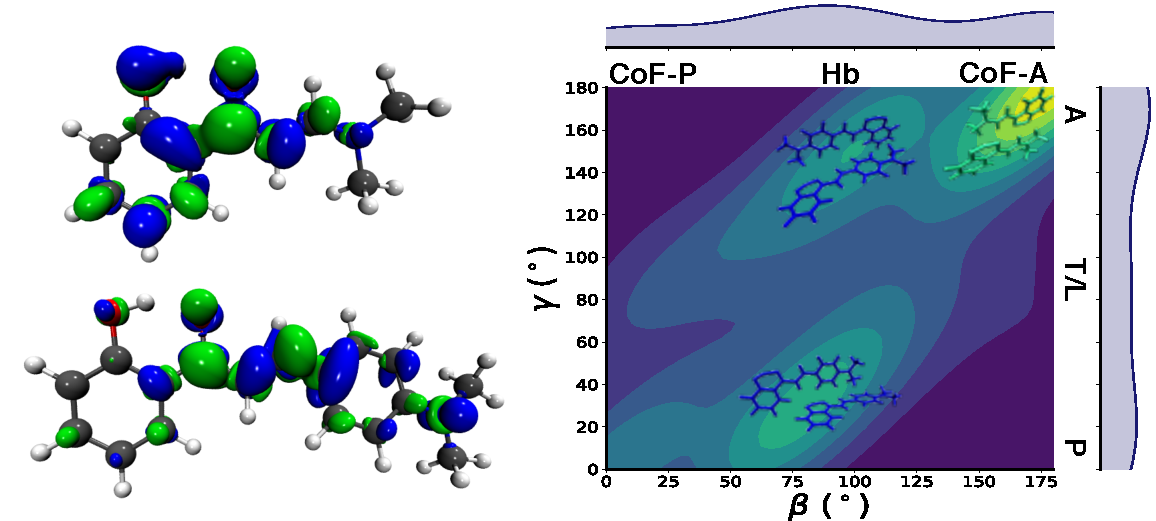
\includegraphics[width=0.7\linewidth]{5ConnectingCrystalStructure/3toc.pdf}
\end{figure}
\section{Introduction}\label{section: Connecting_Introduction}

In Chapters \ref{chapter:NRdecay} and \ref{chapter: Inter} the \acp{PES} of a range of \ac{HC} derivatives were mapped, first in vacuum and then crystalline form. Through the topology of the PESs and the associated energy differences between states, we elucidated the AIE mechanism of \textbf{HC1} and the nonemission of \textbf{HC5}. In doing so, we isolated three key design principles to increase the quantum yield of fluorescence for ESIPT chromophores in the solid state:
\begin{enumerate}
    \item bias for \Kstar{} decay over \Estar{}
    \item localisation of excited state to one monomer 
    \item an energetically inaccessible conical intersection
\end{enumerate}

In this Chapter the scope of the study is extended as these design rules are applied to a new set of ESIPT systems. To the test set we add two fluorine-substituted \ac{HC} derivatives, \ac{HC}\textbf{6} and \textbf{HC7}.\cite{Cheng2016} Additionally, four completely new compounds with lasing properties are considered. Closely related to \acp{HC} are the family of \ac{HP} derivatives.\cite{Tang2016} In contrast to \acp{HC}, and other organic fluorophores, \ac{HP} compounds contain only a single aryl group and have remarkable \ac{QE}, ranging from 0.72-0.84. This has been qualitatively attributed experimentally to the herringbone packing mode and molecular rigidity reducing nonradiative decay. The increased quantum yield of the \acp{HP}, with respect to the \acp{HC}, make them prime candidates to test the efficacy of our  design rules. The eleven compounds studied in this Chapter are summarised in Table \ref{table: chalcones} and shown in Figure \ref{figure: HCHP_structures}.
\begin{figure}[t]
\centering
  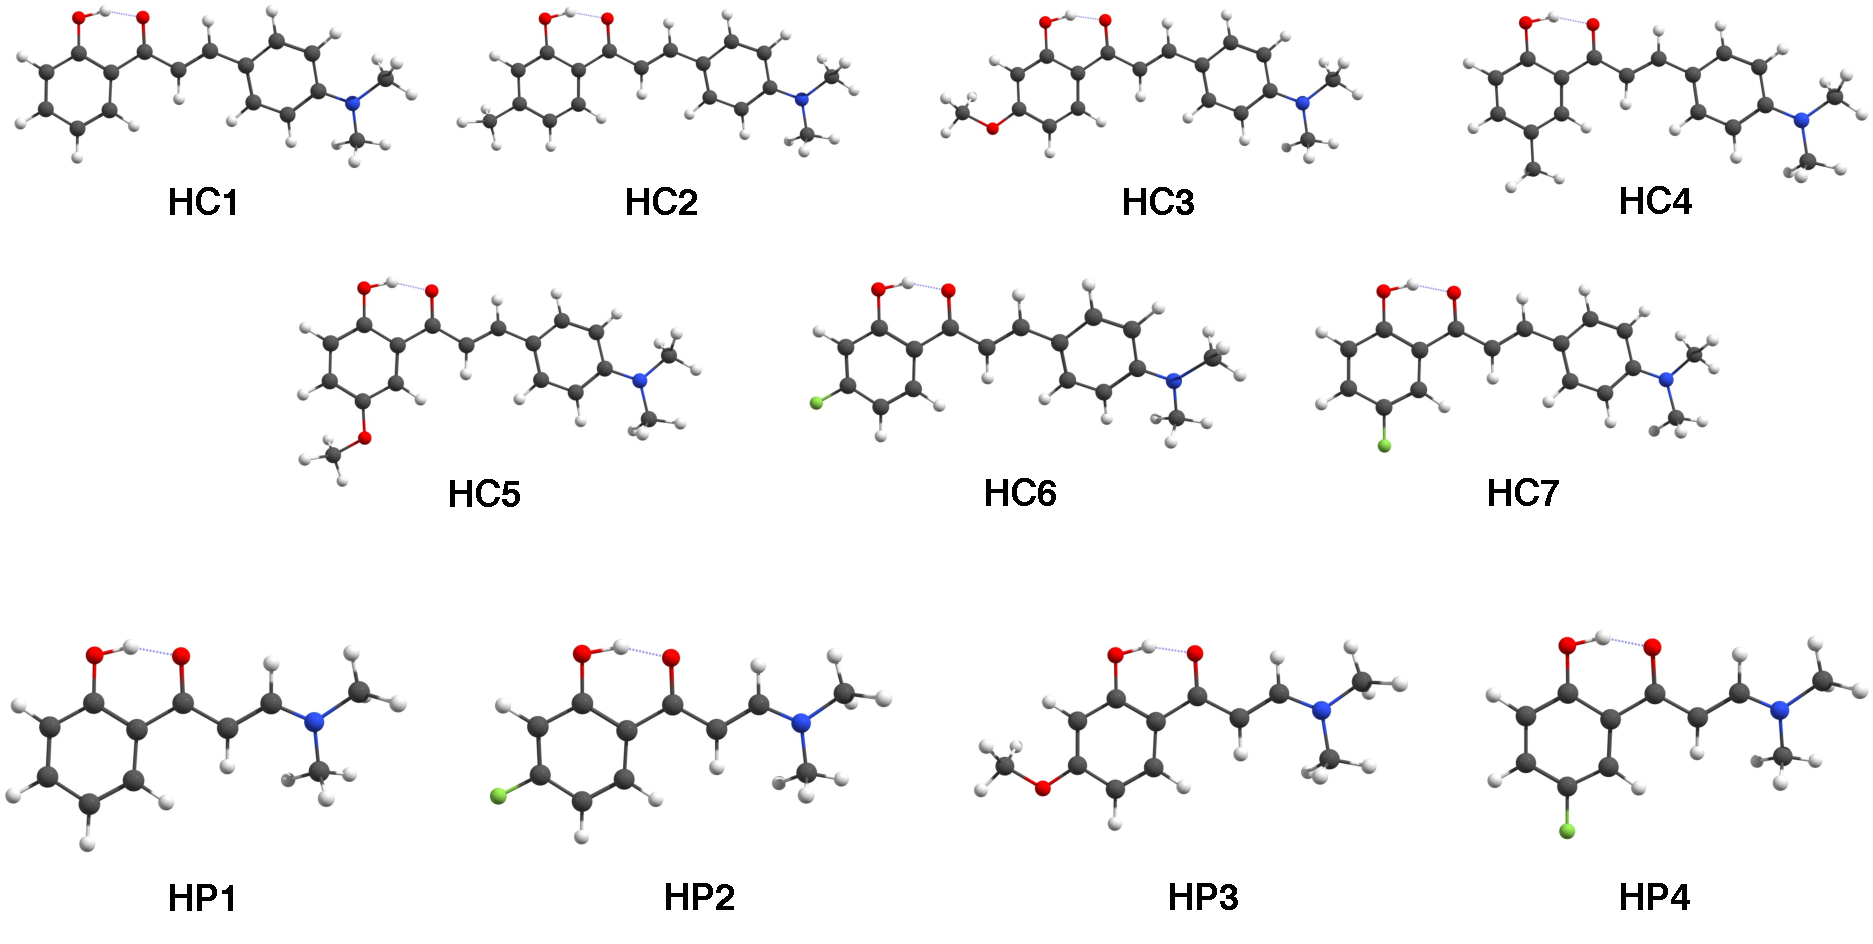
\includegraphics[width=\linewidth]{5ConnectingCrystalStructure/HCHP_structures.pdf}
  \caption[Molecular structures of eleven \textbf{HC} and \textbf{HP} compounds]{The molecular structure of the seven \textbf{HC} and four \textbf{HP} compounds under investigation.}
  \label{figure: HCHP_structures}
\end{figure}
Herein we investigate the factors which mediate the increased fluorescence activity for \textbf{HP} compared to \textbf{HC} systems. In the following sections we address molecular and material properties of the eleven compounds to investigate why the \acp{HP} systems have an increased \ac{QE} compared to their \textbf{HC} counterparts. We will show how a combination of electronic properties and crystal packing give the \textbf{HP} systems an increased potency for each of the three design rules, resulting in increased fluorescence in the solid state. Particular focus will be given to \textbf{HC1}, \textbf{HC5}, and \textbf{HP1}, which will act as exemplar systems due to their differing fluorescence behaviour.

After outlining the computational methods used, we address the molecular properties of the \textbf{HC} systems. We map the \acp{PES} of \textbf{HP1}-\textbf{4} in vacuum, to locate the nonradiative decay channels and gauge the substituent effects, showing how the increased bias for the keto channel promotes \ac{ESIPT} in these systems, fulfilling design rule one. We then move to the crystalline state and show how a stable \Kstar{} minimum and inaccessible conical intersection promote radiative decay in \textbf{HP1}, satisfying design rule three. We compute the radiative decay rates for \textbf{HC1}, \textbf{HC5}, and \textbf{HP1} \textit{via} two methods to compare the exemplar compounds, and examine the Huang-Rhys factors to qualitatively assess the \ac{FGR-RIM} interpretation for nonradiative decay.

We then turn our attention to the intermolecular properties of the eleven molecular crystals. The crystal structures are analysed with particular attention paid to the dimer configurations present. We examine how the dimer arrangements mediate the excitonic coupling between molecular sites in the crystal and afford localisation of the excited state. Following this, an exciton hopping model based on Marcus Theory is applied to examine the different hopping rates in the enol state and examine the competition between localisation and exciton diffusion, and how the \textbf{HP} systems show greater charge localisation to fulfil the second design rule.  All calculations and analyses were performed by myself except for the implementation of the Voronoi cells, which was done by Miguel Rivera, and the TDDFT optimisations in vacuum of \textbf{HP1}-\textbf{4}, which were carried out by Matthew Hollis-Smith. At the time of writing, a manuscript based on this chapter is in the final stages of preparation for publication.

%%%%%%%%%%%%%%%%%%%%% 
%%%%%%%%%%%%%%%%%%%%% 
\section{Computational Details}\label{section: Connecting_Comp}
%%%%%%%%%%%%%%%%%%%%% 
%%%%%%%%%%%%%%%%%%%%% 
Crystal structures of compounds \ac{HC}\textbf{1}-\textbf{7} and \ac{HP}\textbf{1}-\textbf{4} were obtained from the CCDC as described in references{~\citenum{Cheng2015,Cheng2016,Tang2016}}. \ac{HP}\textbf{1}-\textbf{4} were optimised in vacuum in the \szero{} and \sone{} enol and keto states at the (TD-)$\omega$B97X-D/6-311++G(d,p) level of theory. Conical interesctions were optimised at the same level of theory using CIOpt. Relaxed geometry scans of the torsional rotation angle $\theta_{tor}$ in the keto \sone{} state (\Kstar) were performed for the same compounds. Proton migration scans of the ESIPT process were also performed in vacuum for \ac{HC}\textbf{1}, \textbf{HC5} and \ac{HP}\textbf{1}. All scans were calculated at TD-$\omega$B97X-D/6-31G(d). 

Crystal structures of all \ac{HC} and \ac{HP} compounds were optimised using Quantum Espresso in the periodic DFT framework.\cite{QE-2009} Optimisation of each unit cell was carried out with DFT-D2 (PBE) with a plane-wave cutoff of 30 Ry and ensuring Monkhorst-Pack k-point convergence in each case. As the exemplar parent \ac{HP} compound, the full excited state decay mechanism of \ac{HP}\textbf{1} was established through QM:MM cluster models using density functional and multireference methods. A monomer and trimer chromophore at the centroid of the 20{\AA} cluster were optimised in the ground and excited states at ONIOM((TD-)$\omega$B97X-D/6-31G(d):AMBER) level of theory. The \sone/\szero{} MECI in both monomer and trimer cluster models were calculated using a modified version of the CIOpt algorithm.\cite{Levine2008} 

The MECI in the monomer cluster models was also obtained with the state-averaged complete active space self-consistent field method, employing the \szero{} and \sone{} states in the averaging. The active space consisted of 12 electrons in 11 orbitals (SA-2-CASSCF(12,11)). The 6-31G(d) basis set was using for the QM region and the AMBER forcefield was used to describe the MM region. Calculating the MECI with CASSCF:MM ensures the validity of the TD-DFT:MM-calculated MECI. The potential energy profile was refined with multistate complete active space second-order perturbation theory (MS-3-CASPT2(12,11)/6-31G(d):AMBER), incorporating the \szero{}, \sone{}, and \stwo{} states. The TD-DFT:MM geometries from the trimer models at the Franck-Condon, \sone{} minimum, and MECI were taken as the reference geometries, where the central molecule was taken for the CASPT2 calculation and the remaining two molecules of the trimer were added to the MM region.  A three state average was used. The orbitals chosen for the active space are shown in Appendix D. All density functional calculations were performed in the Gaussian 09 suite of programs.\cite{g09} CASSCF and CASPT2 calculations used OpenMolcas with the Tinker v.6.3.3 interface.\cite{Aquilante2016}

Crystalline emission spectra for \textbf{HC1}, \textbf{HC5} and \textbf{HP1} in \Estar{} and \Kstar{} minima were simulated using the nuclear ensemble method as implemented in the NEWTON-X software suite.\cite{Barbatti2014} 100 initial conditions were sampled from the harmonic frequencies calculated at ONIOM(TD-$\omega$B97X-D/6-31G(d)):AMBER level from 7\AA{} cluster models. The \sone{}-\szero{} energy gap was computed for each initial condition in embedded point charges to reflect the positions of the MM charges. No MM-level energies were computed, and as such the fluorescence spectra are of only the electronic energies.

To calculate solid state reorganisation energies in the adiabatic approximation ($\lambda_{A}$, Equation \ref{equation: lambda}) for each compound we generated cluster models based on the 2x2x2 supercell, where all molecules which lay within 20{\AA} of the central monomer chromophore were included in the cluster. Geometries were optimised for all eleven clusters in \sone{} and \szero{} states within the ONIOM protocol at $\omega$B97X-D/6-31G(d):UFF using electrostatic embedding. MM charges were derived automatically using the QEq method.\cite{Rappe2007} The UFF forecefield was chosen here due to the automatic charge assignment, allowing the highthroughput generation of structures and input files. In the cases of \ac{HC}\textbf{1}-\textbf{4} and \ac{HC}\textbf{6}-\textbf{7}, $\lambda_{A}$ was calculated for both enol and keto pathways. For \textbf{HC5} and \textbf{HP1}-\textbf{4}, only the $\lambda_{A}$ associated with keto relaxation was used since no \Estar{} minimum was located in the monomer QM:MM relaxation. Reorganisation energies in the normal-mode approximation ($\lambda_{NM}$) were calculated using the DUSHIN program for \textbf{HC1}, \textbf{HC5} and \textbf{HP1}.\cite{Reimers2001} Frequencies for an ONIOM-optimised monomer chromophore were calculated in an array of point charges representing the molecular crystal, at TD-$\omega$B97X-D/6-31G(d) level. This lead to one imaginary frequency in each case.

Exciton couplings \textit{J} were calculated for dimers in each optimised crystal structure. A 2x2x2 supercell was constructed for each system and a dimer was defined as any molecular pair with an interatomic distance less than or equal to the van der Waals radii of the atoms, plus a damping factor of 1.5\AA. This selection criterion has previously been used in similar applications.\cite{Campbell2017} 

To analyse the spatial environment for the monomers at the centre of the cluster models in the each crystal, Voronoi cells partition the crystal into molecular regions. These cells define all the points in space which are closer to the reference molecule than an exterior molecule. Dividing the Voronoi cell volume by the van der Waals volume gives a molecule-independent Voronoi index $V_{i}$ for each crystal structure. To generate the Voronoi cells, a cluster of molecules was extracted from its crystalline positions. A real space grid was generated at an arbitrary resolution and at each point of this grid, the distance to each atom was calculated and scaled by the corresponding van der Waals radius. All voxels with the lowest scaled distance belonging to an atom of the central molecule were marked as belonging to the accessible of the molecule, resulting in an irregular polyhedron of finite volume.
%%%%%%%%%%%%%%%%%\\
%%%%%%%%%%%%%%%%%
\section{Results}\label{section: Connecting_Results}
%%%%%%%%%%%%%%%%%
\subsection{Potential Energy Surfaces of \textbf{HP} Derivatives in Vacuum} \label{section: Connecting_Vacuum}
The \acf{HP} compounds synthesised by Tang \textit{et al.} show remarkable \ac{AIE} behaviour.  Before studying the root of their fluorescence in the solid state, in this section the \acp{PES} are mapped in vacuum at (TD-)DFT level. This enables the isolation of the substituent effect and to understand the effect of removing an aryl ring from the \ac{HC} structure. 
\begin{figure}[t]
\centering
  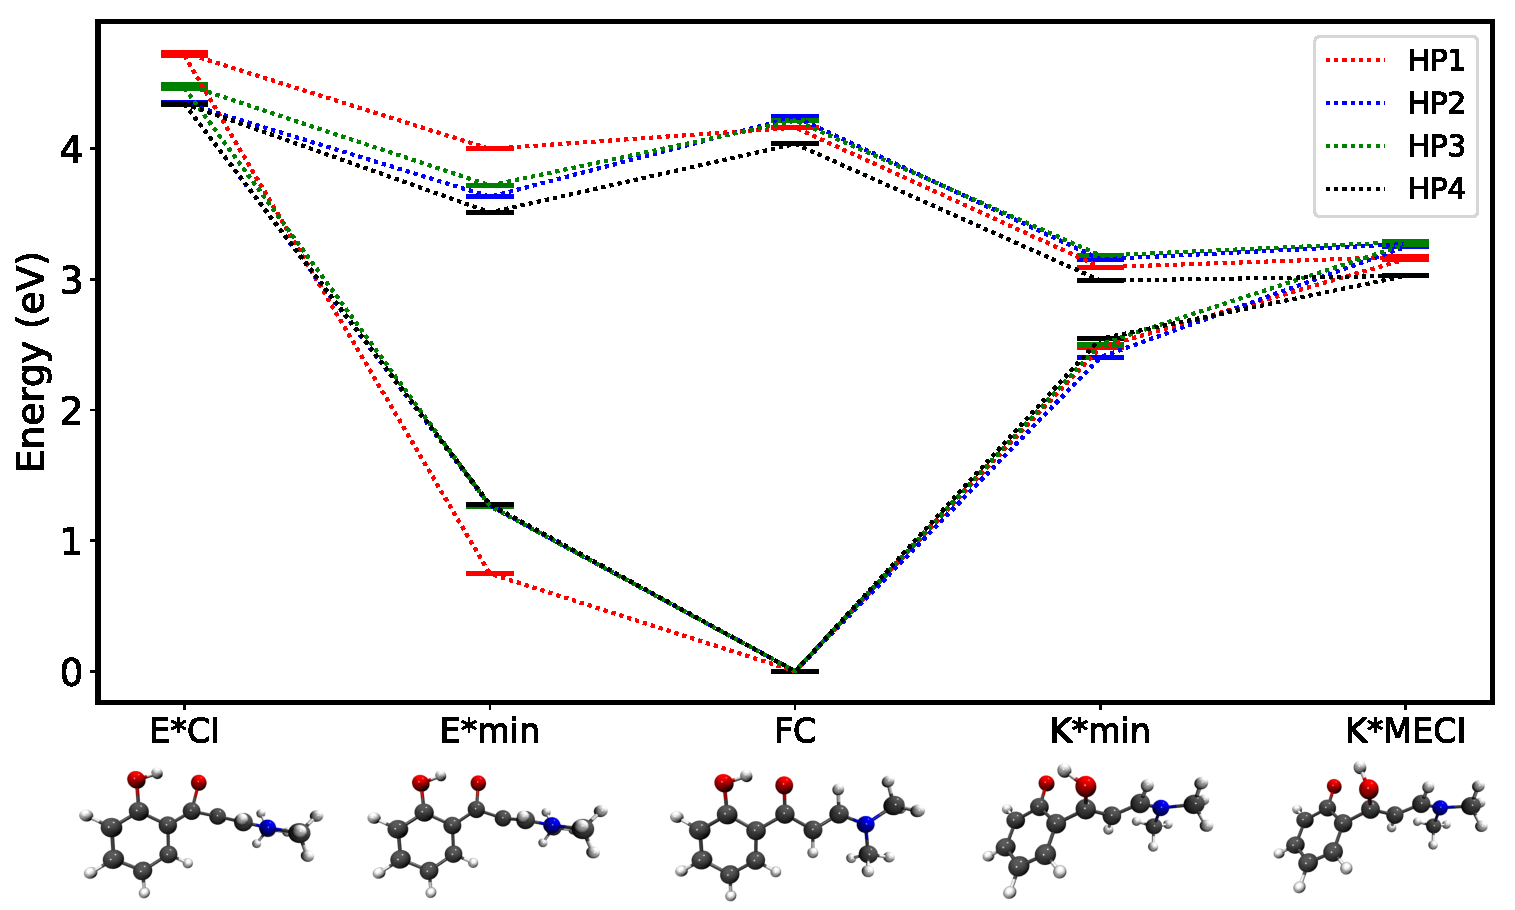
\includegraphics[width=0.8\linewidth]{5ConnectingCrystalStructure/2HP_energies_vac.pdf}
  \caption[The vacuum PES of HP\textbf{1}-\textbf{4} with TDDFT]{The critical points on the \ac{PES} for \textbf{HP}\textbf{1}-\textbf{4} obtained at (TD-)$\omega$BX-D/6-311++G(d,p) in vacuum. Also shown are the optimised geometries at each point for \textbf{HP1}.}
  \label{figure: HP_energies_vac}
\end{figure}

In Figure \ref{figure: HP_energies_vac}, the energy levels of the key regions of the \ac{PES} are shown for \textbf{HP1}-\textbf{4}. Vertical excitation to \sone{} in vacuum is predicted at 4.16 eV for \textbf{HP1}, a blue shift of 0.51 eV compared to \textbf{HC1}.  There is a blue shift of 0.09 eV for \textbf{HP2} and a red shift of 0.18 for \textbf{HP4} compared to \textbf{HP1}. These excitations are all  bright and HOMO-LUMO in character. The difference density plots show that density is lost from the phenol oxygen and donated to the C=O carboynl, as for \sone{} in \textbf{HC5} (Figure \ref{figure: monomer_excitations}). Results from Chapter \ref{chapter:NRdecay} show that this electronic structure promotes ESIPT. In \textbf{HP2} and \textbf{HP3}, there is some donation from the amino N. In \textbf{4}, electron density is lost from the fluorine. 

The experimental absorption in DCM is centred at 3.43 eV for \textbf{1}, and thus the TDDFT excitation energies are largely overestimated. When a solvent cavity is introduced through the \ac{PCM} model, the \sone{} energy is red shifted to 4.01 eV - an improvement but still largely overestimated compared to experiment. It is for this reason that in the solid state calculations in Section \ref{section: Connecting_Relaxation}, the CASPT2 method is applied to determine the energetic pathways.
\begin{figure}[t]
\centering
  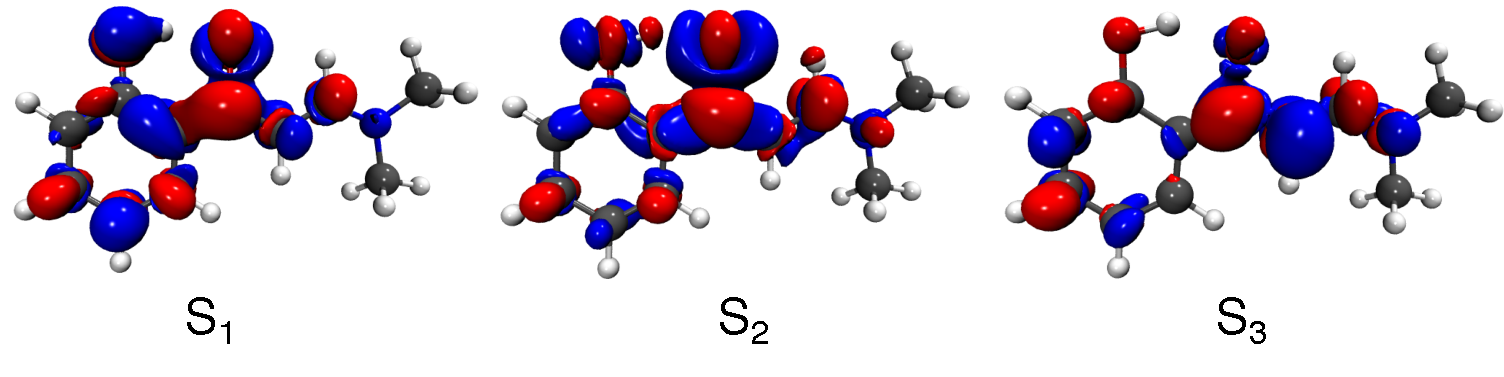
\includegraphics[width=0.9\linewidth]{5ConnectingCrystalStructure/monomer_excitations.pdf}
  \caption[Electron density difference maps for the first three excitations of \textbf{HP1}.]{Electron density difference maps for the first three excitations of \textbf{HP1}. Blue regions represent electron density loss from the ground state and red represent electron density gain in the excited state, with isovalue of 0.002. Calculated at TD-$\omega$B97X-D/6-311++G(d,p) in vacuum.}
  \label{figure: monomer_excitations}
\end{figure}

In the enol channel relaxation is not \textit{via} rotation about $\theta_{tor}$, instead occuring through partial cis-trans isomerisation about the carbon-carbon double bond. Fluorescence from this state is dipole forbidden with negligible oscillator strength. The conical intersection on the enol channel is inaccessible, with a distortion of the carbonyl group. 

The relative energetic stability of the keto channel is expected to result in a large bias and high population of \Kstar{}. As for the \textbf{HC} systems, relaxation is \textit{via} rotation about $\theta_{tor}$ (defined in Figure \ref{figure: dihedral_scans_vac}) and is heavily favoured, as shown by the relaxed geometry scan of $\theta_{tor}$ in Figure \ref{figure: HP_scan_vac}. There is destablisation of the ground state through the rotation but the keto state remains stable through 180\degree{}. We shall return to this concept in Section \ref{section: Connecting_Bias}. Full isomerisation is not expected due to the high energy of the trans-keto state in both \sone{} and \szero{} compared to the cis-keto conformer. The conical intersection is energetically accessible in vacuum, with the substituent effects relatively minor. This is to be expected, since experimental results show that both absorption and emission energies show only minor (\textless{} 0.15 eV) substituent dependence. 

\begin{figure}[t]
\centering
  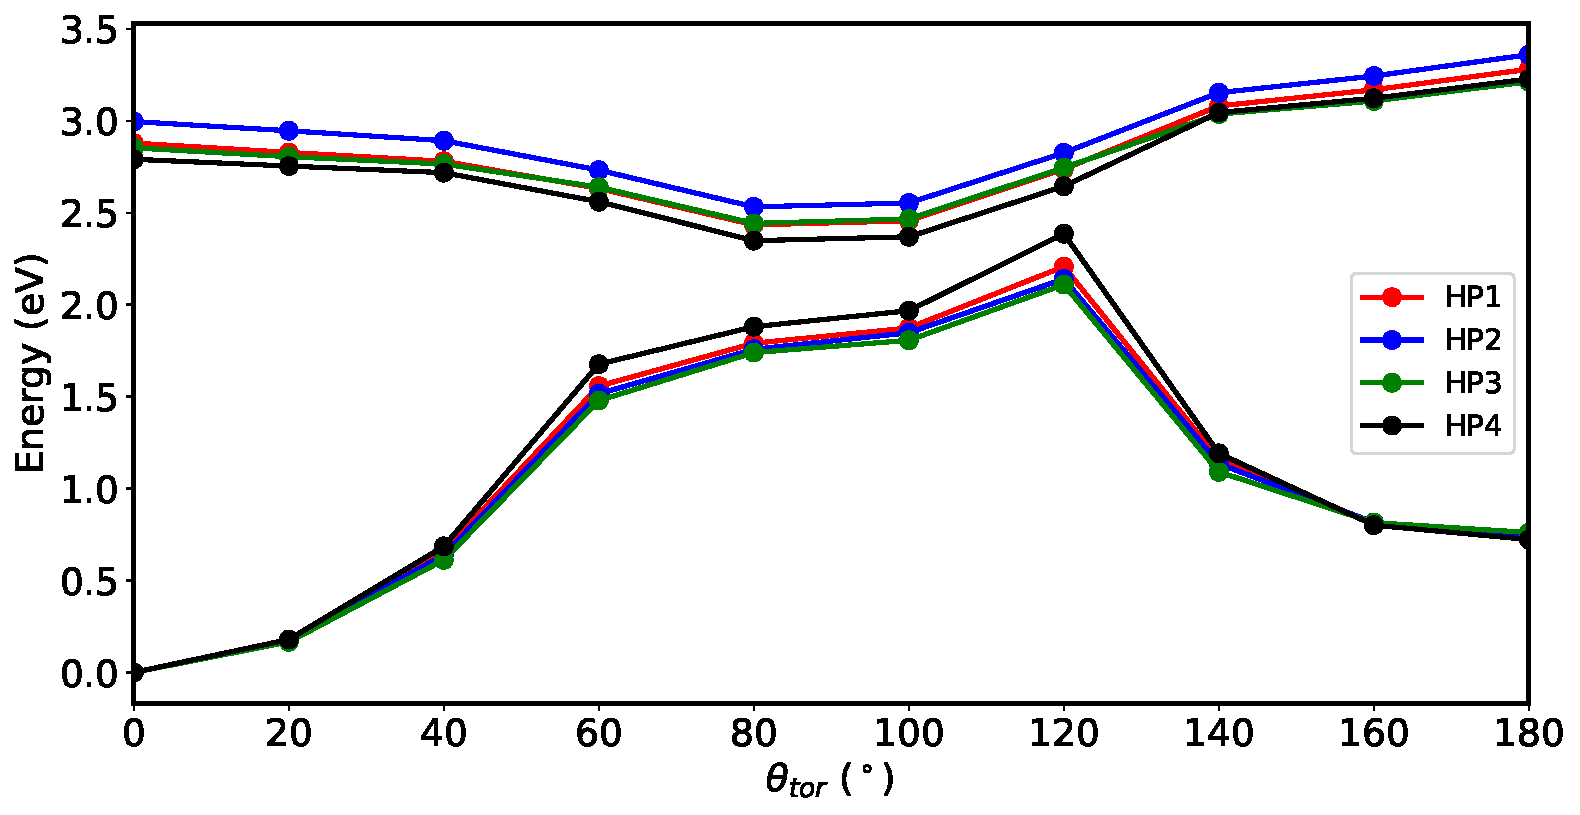
\includegraphics[width=0.9\linewidth]{5ConnectingCrystalStructure/2HP_scan_vac.pdf}
  \caption[Relaxed geometry scan of $\theta_{tor}$ for \textbf{HP} derivatives]{Relaxed geometry scan of $\theta_{tor}$ for \textbf{HP1}-\textbf{4}, calculated at TD-$\omega$B97X-D/6-31G(d) level of theory in vacuum.}
  \label{figure: HP_scan_vac}
\end{figure}
%%%%%%%
%%%%%%%
\subsection{\textbf{HP} Bias for ESIPT}\label{section: Connecting_Bias}
%%%%%%%
%%%%%%%
In this section, it is shown that the \Kstar{} population is enhanced by the inherent bias for ESIPT in the \textbf{HP}s compared to the \textbf{HC}s. The electronic densities show that in the bright excitation of \textbf{HC1}, electron density is mainly donated from the unsaturated bridge and the dimethylaniline moeity (Figure \ref{figure: monomer_excitations}). In contrast, in \textbf{HC5} and to a greater extent \textbf{HP1} (due the removal of the second aryl group), electron density is decreased at the phenol oxygen in the excited state (Figure \ref{figure: HC_Vac_Densities}). NBO charge analysis of the phenol oxygen shows that $\Delta$q increases from +0.01 to +0.05 to +0.09 for \textbf{HC1}, \textbf{HC5} and \textbf{HP1} respectively. This increases the bias for ESIPT in \textbf{HC5} and \textbf{HP1} due to the increased acidity of the transferring proton, as shown by the excited state PES relaxed geometry scan in Figure \ref{figure: Hscan}. \textbf{HP1} shows a stabilisation of 0.62 eV, compared to 0.48 eV for \textbf{HC5} and 0.38 for \textbf{HC1}. 

\begin{figure}[t]
\centering
  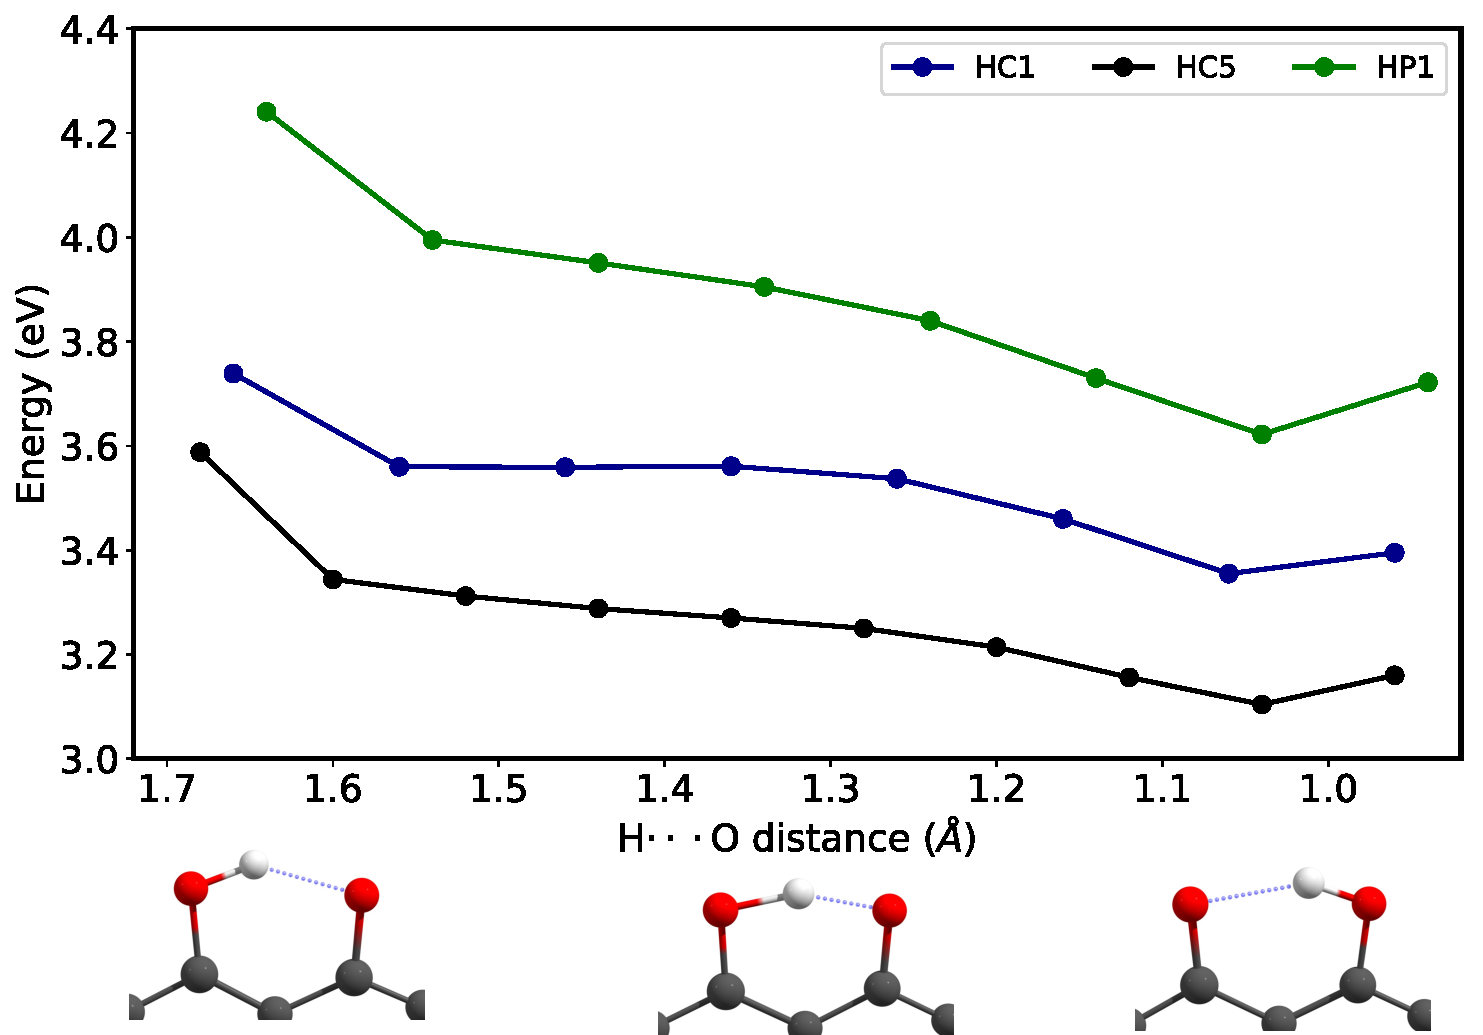
\includegraphics[width=0.8\linewidth]{5ConnectingCrystalStructure/Hscan}
  \caption[Relaxed geometry scan for ESIPT process.]{Relaxed geometry scan of the phenol hydrogen to carbonyl oxygen distance for \textbf{HC1}, \textbf{HC5} and \textbf{HP1}, calculated at TD-$\omega$B87X-D/6-31G(d). Electron density difference maps are also shown, where blue represents electron density loss in \szero{} and red is electron density gain in \sone{}.}
  \label{figure: Hscan}
\end{figure}

In the \Kstar{} channel in vacuum, relaxed geometry scans along the torsional relaxation mode (Figure \ref{figure: dihedral_scans_vac}) show that for \textbf{HC5}, the onset of the conical intersection seam is reached at 60\degree, due to the overload of electronic density at the protonated carbonyl group. Contrastingly in \textbf{HP} systems, the conical intersection seam is not found along torsional relaxation mode. While the electronic density distribution in \textbf{HP} systems leads to a strong bias for ESIPT, as for \textbf{HC5}, it does not destabilise the ground state during rotation to the same extent. \textbf{HP} systems are thus inherently more stable in the \Kstar{} channel. However, for all \textbf{HC} and \textbf{HP} systems, the MECI in non-aggregated form is energetically accessible post photoexcitation and thus nonradiative decay is witnessed experimentally. The proton lability in the \textbf{HP} systems on accountelectron density distribution, and the stability of the \Kstar{} minimum, means they obey design rule one more strictly than in the \textbf{HC} systems. 

\begin{figure}[t]
\centering
  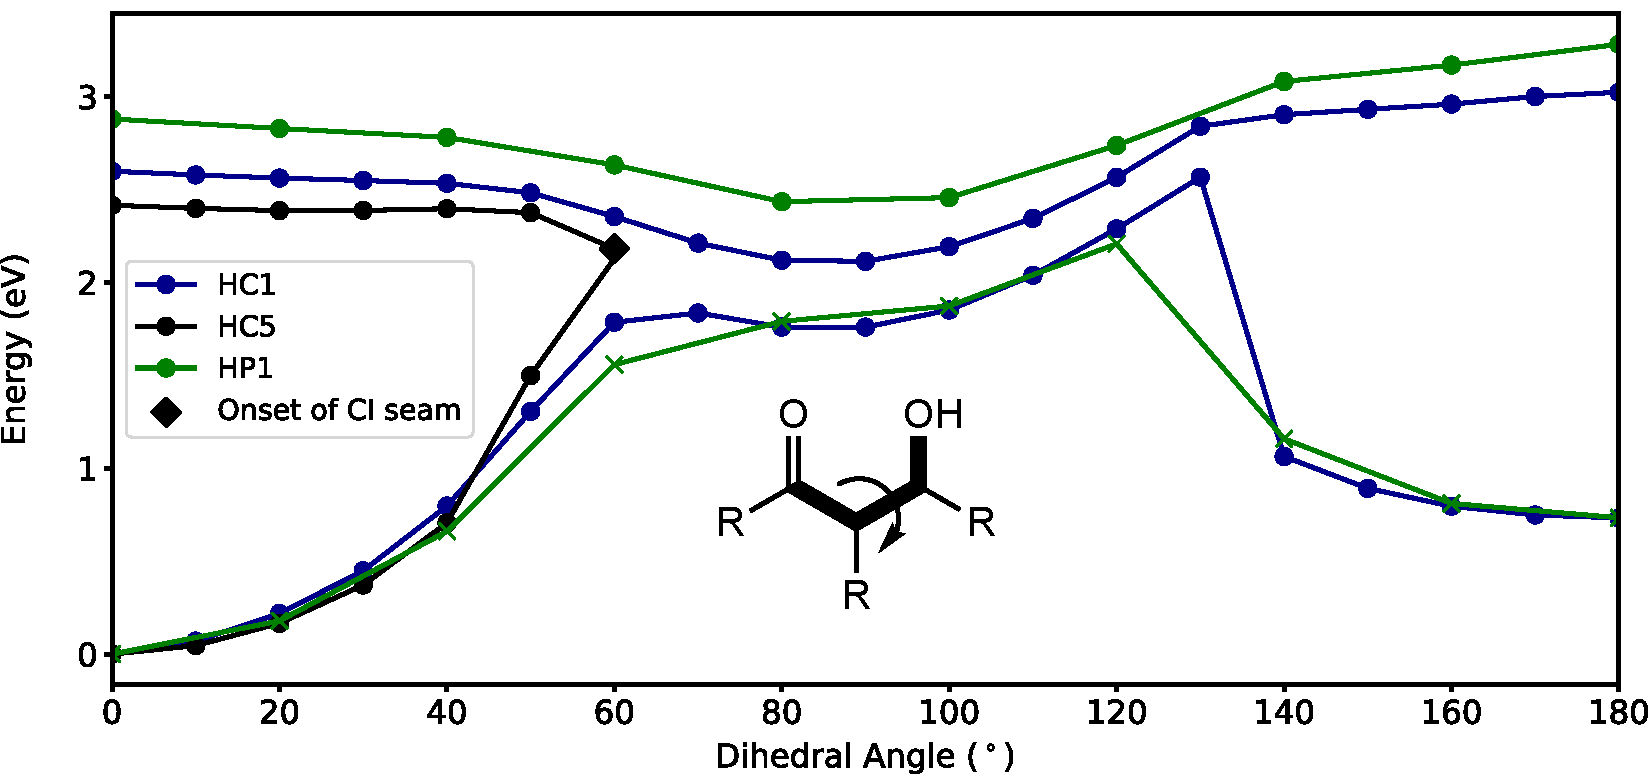
\includegraphics[width=0.8\linewidth]{5ConnectingCrystalStructure/dihedral_scans_vac}
  \caption[Relaxed geometry scan of the torsional angle]{Relaxed geometry scan of the torsional angle (shown inset, $\theta_{tor}$)  for \textbf{HC1}, \textbf{HC5} and \textbf{HP1} in vacuum, calculated at TD-$\omega$B87X-D/6-31G(d). For \textbf{HC5}, the scan cannot proceed further than 60\degree{} due to the convergence of the two electronic states.}
  \label{figure: dihedral_scans_vac}
\end{figure}

%%%%%%%%%%%%%%%%%%%%%%%%
%%%%%%%%%%%%%%%%%%%%%%%%
\subsection{Relaxation Pathways in the Molecular Crystal}\label{section: Connecting_Relaxation}
%%%%%%%%%%%%%%%%%%%%%%%%
%%%%%%%%%%%%%%%%%%%%%%%%
Results from Chapter \ref{chapter: Inter} showed that efficient population transfer to the \Kstar{} tautomer is only one prerequisite for fluorescence. The accessibility of the nearest conical intersection can dictate the luminescent response. For \textbf{HC1}, fluorescence is possible due to the high energy conical intersection in the solid state. On the other hand, for \textbf{HC5}, whilst ESIPT is more efficient than in \textbf{HC1}, the \ac{QE} is essentially zero and AIE is not seen. This can be attributed to dominance of nonradiative decay as a result of a low-lying MECI being classically accessible post electronic excitation. While intermolecular factors play a role in the conformation of the MECI, the energetic accessibility is determined by the electronic structure of the chromophore. To asses the accessibility of the MECI in the solid-state in \textbf{HP1}, we construct the excitation-decay pathway in the using QM:MM cluster models. The calculated PES for \textbf{HP1} in vacuum and the solid state is shown in Figure \ref{figure: HP1_crystal_vs_vac}.
Geometries were optimised at the Franck-Condon, the \Kstar{} minimum and the MECI with (TD-)$\omega$B97X-D/6-31+G(d):AMBER using a trimer chromophore. The central monomer, where ESIPT and the MECI occur, was then used as the chromophore in MS-3-CASPT2(12,11)/6-31G(d):AMBER single point calculations, with the two other members of the trimer demoted to the MM-level. This eased the computational expense in the MS-3-CASPT2(12,11):AMBER calculations, which are necessary to accurately predict the energy of the \sone{} excitation in the solid state. The MECI geometry obtained with TD-DFT is verified through comparison with MS-2-CASSCF(12,11):AMBER.
%%%
\begin{figure}[t]
\centering
  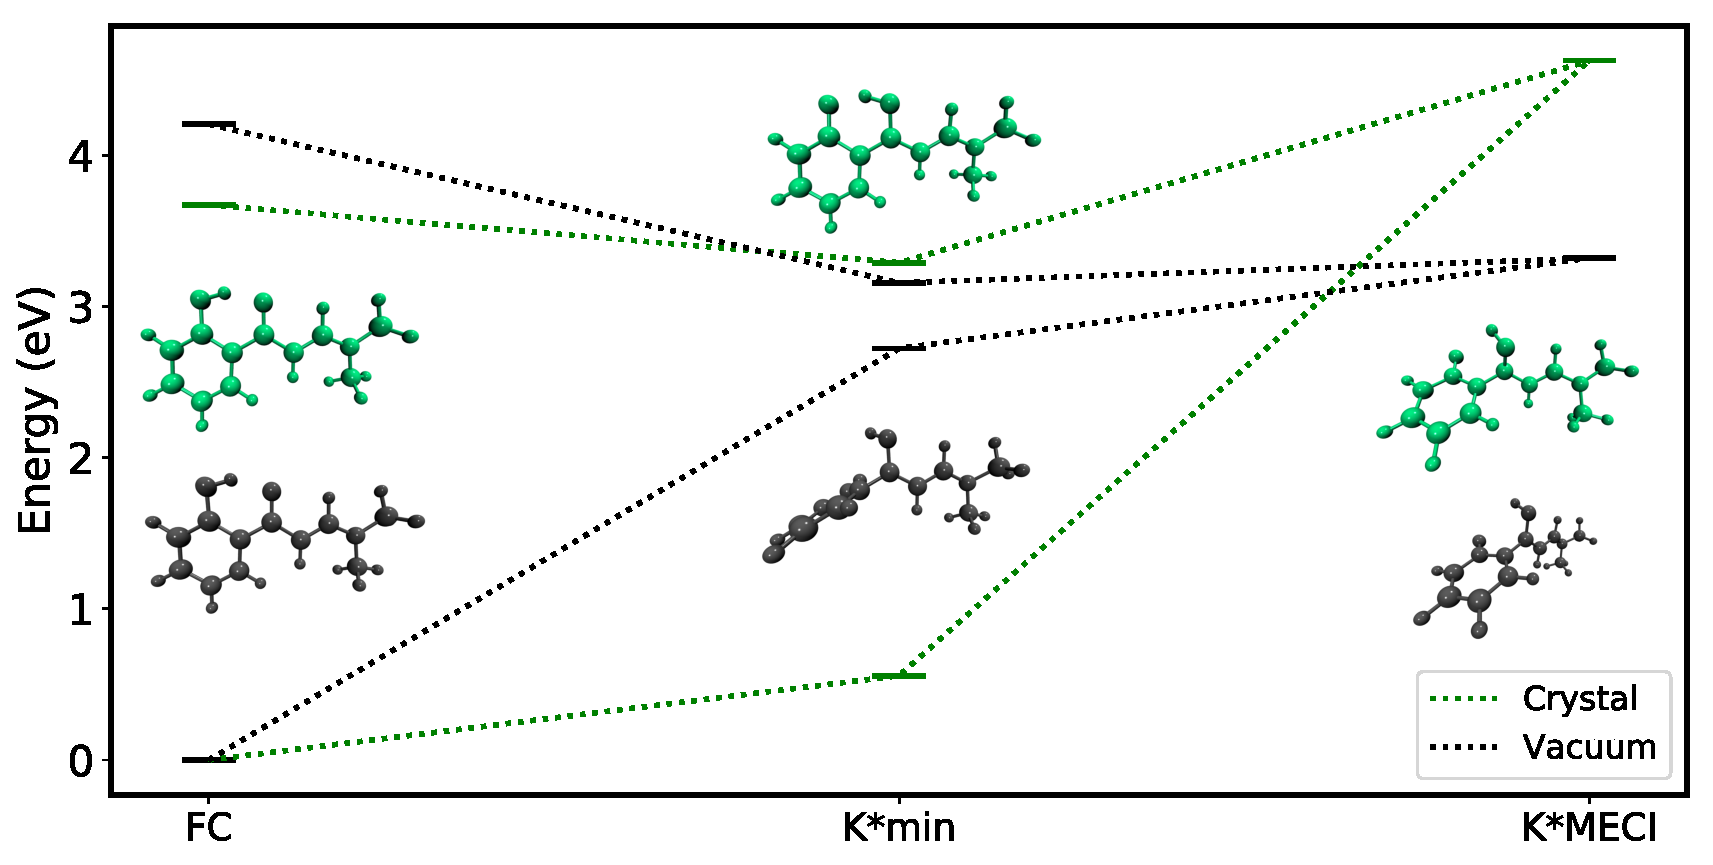
\includegraphics[width=0.9\linewidth]{5ConnectingCrystalStructure/HP1_crystal_vs_vac}
  \caption[PES for \textbf{HP1} in vacuum and the solid state]{Calculated energies and geometries at critical points on PES. Geometries obtained with (TD)-$\omega$B97X-D/6-31G(d)(:AMBER), with energies calculated at MS-3-CASPT2(12,11):(AMBER). The average energy of the \sone{} and \szero{} states is shown for the MECI.}
  \label{figure: HP1_crystal_vs_vac}
\end{figure}
%%%
At the MS-3-CASPT2(12,11)/6-31G(d):AMBER level, absorption for \textbf{HP1} is calculated at 3.67 eV (\textit{f}=0.868), in fair agreement but blue-shifted by 0.41 eV compared with the crystalline absorption maximum of 3.26 eV.\cite{Tang2016} 
With a four-state average (MS-4-CASPT2), this improves further to 3.52 eV. With TD-$\omega$B97X-D/6-31G(d):AMBER, the bright state is calculated at 4.25 eV in the trimer model and 4.23 eV in the monomer model, a large overestimation of the absorption energy. When the 6-311++G(d,p) basis set is used, the prediction is slightly improved with the bright state occurring at 4.10 eV. The accurate prediction of the initial photoabsorption is crucial in understanding the excited state mechanism and as such we proceed with using MS-3-CASPT2(12,11)/6-31G(d):AMBER for the energies (which is denoted CASPT2 for brevity). %perhaps the gap between s1 and s2 can be discussed

Post photo-excitation, relaxation in \sone{} \textit{via}  ESIPT is expected to be dominant relaxation channel in \textbf{HP1} due to the negligible oscillator strength (\textit{f}=0.016) of the \stwo{} state, which is n$\pi^\ast{}$ in character. Fluorescence in the molecular crystal is centred at 2.34 eV, thus displaying a Stokes shift of 0.94 eV. The emission wavelength predicted at CASPT2 is 2.73 eV, again in fair agreement and with similar blue-shift as calculated for absorption. Certainly, allowing relaxation of the exterior atoms and mutual polarisation would allow further geometric relaxation and a more accurate emission energy. Also, addition of Ewald point charges to reflect the periodicity of the crystal would improve emission further. However, this was outside the scope of the current work.
%The Stokes-shift is underestimated compared to experiment by 0.5 eV, which can be partially attributed to the frozen MM atoms and neglect of charge relaxation in the excited state.

The MECI in \textbf{HP1} lies 1.46 eV above the \Kstar{} minimum and 1.08 eV above the bright absorption state. As such, it is classically inaccessible and \textbf{HP} emission can be attributed to the trapping of the excited state at the \Kstar{} minimum, followed by radiative decay. The degeneracy of the \sone{} and \szero{} states on going from CASSCF to CASPT2 is lifted slightly, with a gap of 0.2 eV at CASPT2 level. As the substituent effects in the crystalline samples are minor in the \textbf{HP} samples (absorption and fluorescence), it can be assumed that this mechanism can be applied to all four systems in the family. It would be of interest to synthesise a \textbf{HP} system with a methoxy group the \textit{para} position, as in \textbf{HC5}, to assess its AIE behaviour.

In Figure \ref{figure: MECI_comparison}, the MECI geometries of \textbf{HC1}, \textbf{HC5}, and \textbf{HP1} are compared. All three involve the pyramidalisation of the protonated carbonyl group  combined with torsional rotation of the deprotonated phenol moeity. In \textbf{HC1} and \textbf{HP1}, the compounds which undergo AIE due to the high energy of the MECI, the torsional angles are 50\degree{} and 53\degree{} respectively. In \textbf{HC5}, where the MECI is energetically accessible, the pyramidal distortion is only 28\degree{}. The same effect is seen in vacuum, where the MECI of \textbf{HC5} is also onset at lesser distortion than the other systems, as discussed above. Thus the stability of the \textbf{HC5}, and the high energy MECIs of \textbf{HC1} and \textbf{HP1}, are mainly due to the electronic effects of the chromophore. Rather, the role of the packing and the crystalline environment as a whole is to promote efficient localisation of the excited state at the expense of exciton hopping the enol state, as will be investigated in Section \ref{section: Connecting_Marcus}. Such is the propensity for localisation and ESIPT in \textbf{HP} and the high energy MECI, a largely increased \ac{QE} is witnessed as a result, fulfilling design rules two and three.
%%%
\begin{figure}[t]
\centering
  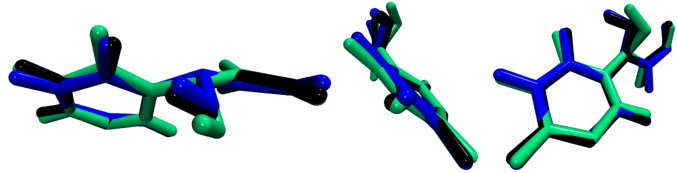
\includegraphics[width=0.9\linewidth]{5ConnectingCrystalStructure/MECI_comparison.pdf}
  \caption[MECI geometries for \textbf{HC1},\textbf{HC5} \% \textbf{HP1}.]{Overlaid structures of the MECI for \textbf{HC1} (blue) and \textbf{HC5} (black), and \textbf{HP1} (green), shown from three viewpoints. Only the atoms shared by all three compounds are shown.}
  \label{figure: MECI_comparison}
\end{figure}

%%%%%
\subsection{Radiative Decay Rates}\label{section: connecting_radiative_rates}
%%%%%
In this section we calculate the emission rate $k_{r}$ for \textbf{HC1}, \textbf{HC5}, and \textbf{HP1}. This can be done either through the Einstein spontaneous emission relationship (Equation \ref{equation: Einstein_rate}) or through integrating the simulated spectrum (Equation \ref{equation: integrated_emission_rate}). The oscillator strength between \sone{} and \szero{} states at the \Kstar{} minimum is 0.549 at CASPT2 level (0.281 TDDFT trimer model,0.331 with TDDFT monomer), indicating that emission will be bright. First, we compute the radiative decay rates from the E* and K* states using ONIOM(TDDFT) by computing the fluorescence spectrum and calculating $k_{r}$ through Equation \ref{equation: integrated_emission_rate}. The spectra for \textbf{HC1}, \textbf{HC5} and \textbf{HP1} are given in Figure \ref{figure: HC1_HC5_HP1_emission_oniom} and radiative rates for \textbf{HC1}, \textbf{HC5} and \textbf{HP1} are given in Table \ref{table: rates}.

\begin{figure}[t]
\centering
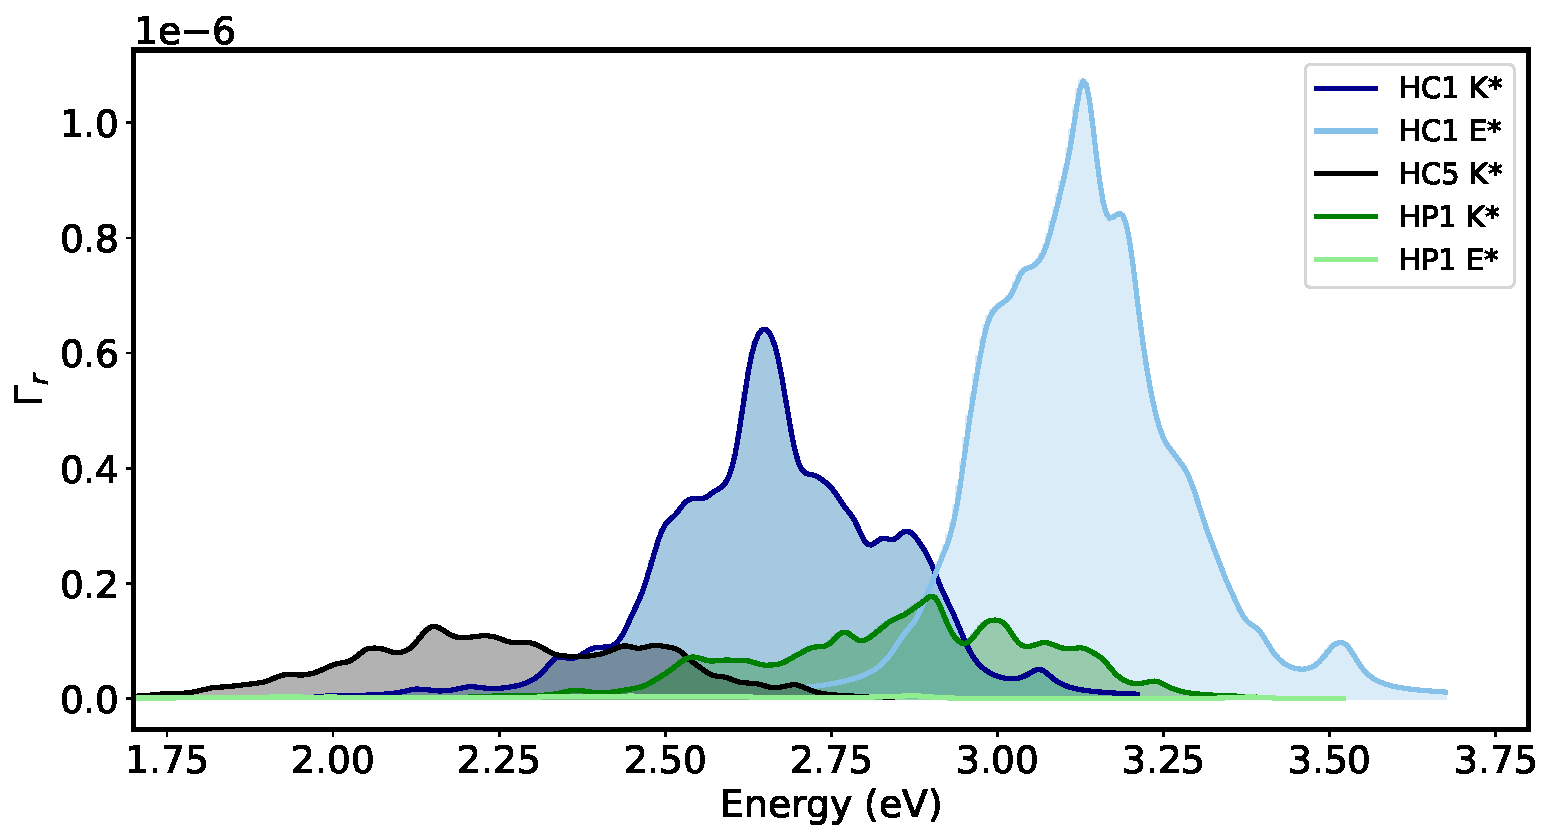
\includegraphics[width=0.8\linewidth]{5ConnectingCrystalStructure/HC1_HC5_HP1_emission_oniom}
\caption[Emission spectra in molecular crystal for 7\AA{} clusters for \textbf{HC1}, \textbf{HC5} and \textbf{HP1}]{Emission spectra in molecular crystal for 7\AA{} clusters for \textbf{HC1}, \textbf{HC5} and \textbf{HP1}, calculated at TD-$\omega$B97X-D/6-31G(d) in point charges. Single point energies were calculated for 100 initial conditions based upon a Wigner distribution of the excited state frequencies calculated at ONIOM(TD-$\omega$B97X-D/6-31G(d):AMBER) level.}
\label{figure: HC1_HC5_HP1_emission_oniom}
\end{figure}

For \textbf{HC1}, $k_{r,K*}$ is comparable with \textbf{HP1} in both E* and K*. However, \textbf{HC1} exhibits lower quantum efficiency, owing to the competing exciton hopping in the enol state, which will inhibit localisation and thus ESIPT. Thus in \textbf{HC1} there is competition between delocalisation, emission from E*, and emission from K*. Due to the proximity of the E* band to the absorption, only K* fluorescence will significantly contribute to the quantum yield.

For \textbf{HP1}, emission from E* is negligible and emission is expected from the K* state. The highly distorted E* minimum, as discussed in the previou section, is expected to play little role in the photochemistry and population transfer to K* should dominate. The radiative rate from K* is of similar magnitude to \textbf{HC1}, and as such the higher quantum yield of \textbf{HP1} is on account of the lower nonradiatve decay rate and lack of other competitive pathways, such as exciton hopping. In Table \ref{table: rates}, given in parenthesis are the rates obtained from the more simple Einstein relationship. This method compares well to the more complex spectral method, where the Wigner distribution of geometries based on harmonic frequencies should certainly provide a more realistic radiative rate. Based on these rates the Einstein relationship can provide a qualitative estimate for $k_{r}$ without the need for computing the fluorescence spectrum, which is a far more computationally demanding approach. However, that is most likely due to the fact that in these systems, the steric hindrance of the molecular crystal means there is little geometric relaxation and the excited state \ac{PES} resembles the ground state \ac{PES}, since there is not the steric freedom to explore outside of the harmonic potential.

\begin{table}
\centering
\caption[Radiative decay rates in the solid state]{Radiative decay rates $k_{r}$ in the solid state in the enol (\Estar{}) and keto (\Kstar{}) regimes for \textbf{HC1}, \textbf{HC5}, \textbf{HP1} calculated through spectral integration. In parenthesis is the rate calculated \textit{via} the Einstein relationship of Equation \ref{equation: Einstein_rate}. All rates in \SI{}{s^{-1}}.} 
\label{table: rates}
  \begin{tabular}{ccc}
    \hline
  	System & $k_{r,E*}$ & $k_{r,K*}$\\
    \hline
    \textbf{HC1} & \SI{4.68e8}{}  (\SI{1.78e9}{}) & \SI{2.99e8}{} (\SI{2.83e8}{}) \\ 
	\textbf{HC5} & - & \SI{9.54e7}{} (\SI{1.02e8}{})\\
	\textbf{HP1} & \SI{5.58e6}{} (\SI{4.49e6}{}) & \SI{1.10e8}{} (\SI{1.23e8}{}) \\
    \hline
  \end{tabular}
\end{table}
%%%%%%%%%%%%%%%%%%
%%%%%%%%%%%%%%%%%%
\subsection{Huang-Rhys Factors}\label{section: HR}
%%%%%%%%%%%%%%%%%%
%%%%%%%%%%%%%%%%%%
As discussed in Section \ref{section: lom HR}, reorganisation energies and \acf{HR} factors are often used to qualitatively account for the \ac{FGR-RIM} interpretation of \ac{AIE}. In this section we address this model for the \textbf{HC} and \textbf{HP} systems.  The \ac{HR} factors in vacuum and molecular crystals were calculated for \textbf{HC1}, \textbf{HC5}, and \textbf{HP1}. In vacuum, ground and excited states were optimised at (TD-)$\omega$B97X-d/6-31G(d) level. In the molecular crystal, a cluster model consisting of a central chromophore and all molecules within a 7\AA{}, taken from the optimised unit cell for each system (see main text for unit cell optimisation details). Ground and excited states were optimised at ONIOM((TD-)$\omega$B97X-d/6-31G(d):AMBER) level, and frequencies were calculated at (TD-)$\omega$B97X-d/6-31G(d) level using point charge embedding. The DUSHIN program was used to calculate the Huang-Rhys factors and the associated reorganisation energies ($\lambda_{NM}$).\cite{Reimers2001}

For \textbf{HP1} and \textbf{HC5}, it is found that $\lambda_{NM}$ overestimates the reorganisation energy with respect to $\lambda_{A}$. In \textbf{HP1},  $\lambda_{A}$ is 1.24 eV compared to 2.19 eV for $\lambda_{NM}$. In \textbf{HC5}, the NM approximation is 0.4 eV larger than $\lambda_{A}$. In both \textbf{HP1} and \textbf{HC5}, the HR factors are reduced in moving from vacuum to the solid state, in particular for rotational modes. The RIM interpretation of AIE prescribes that switch-on of fluorescence upon aggregation is due to dampening of rotational modes, which dissipate the excited state nonradiatively, as witnessed by a reduction in the HR factors. While \textbf{HC1}, \textbf{HC5} and \textbf{HP1} show this effect, \textbf{HC1} and \textbf{HP1} show AIE while \textbf{HC5} is dark in both dispersed and aggregated forms. The dampening of the HR factors does not result in luminescence in \textbf{HC5}, suggesting that the excited state wavepacket decays through the MECI.\cite{Dommett2017} Furthermore, due to the anharmonicity of the PES, the validity of the scheme in these cases is not clear.

To explore this further, Figures \ref{figure: HC1_DUSHIN}-\ref{figure: HP1_DUSHIN} show the Huang-Rhys (HR) factors in vacuum and solid state for \textbf{HC1}, \textbf{HC5} and \textbf{HP1}. The different y-axis scales for the Huang-Rhys factors between plots should be noted. Each system is discussed in turn below.

For \textbf{HC1} in vacuum (Figure \ref{figure: HC1_DUSHIN}, left), the geometric similarity between the planar E* excited state minimum and the ground state equilibrium geometry yields negligible HR factors. This leads to $\lambda_{NM}$ of 0.08 eV, which underestimates the $\lambda_{A}$ of 0.36. For K*, the PES in vacuum is highly anharmonic, and intramolecular rotation leads to a highly distorted geometry with respect to the ground state. As a consequence, the HR factors are extremely large and the harmonic approximation is non-applicable for determining the reorganisaiton energy, as shown by a value of 99 eV ($\lambda_{A}$=3.64 eV). Moving to the molecular crystal (Figure \ref{figure: HC1_DUSHIN}, right), in E* the HR factors are of similar magnitude as in vacuum but in K* they are markedly reduced and suppressed to fractional values. The largest K* HR factor is the O-H stretching mode, since the geometry remains planar and has the largest displacement between \szero{} and \sone{} as it is the ESIPT coordinate. The K* $\lambda_{NM}$ is 4.67 eV, with $\lambda_{A}$=0.59 eV. 

\begin{figure}[t]
\centering
  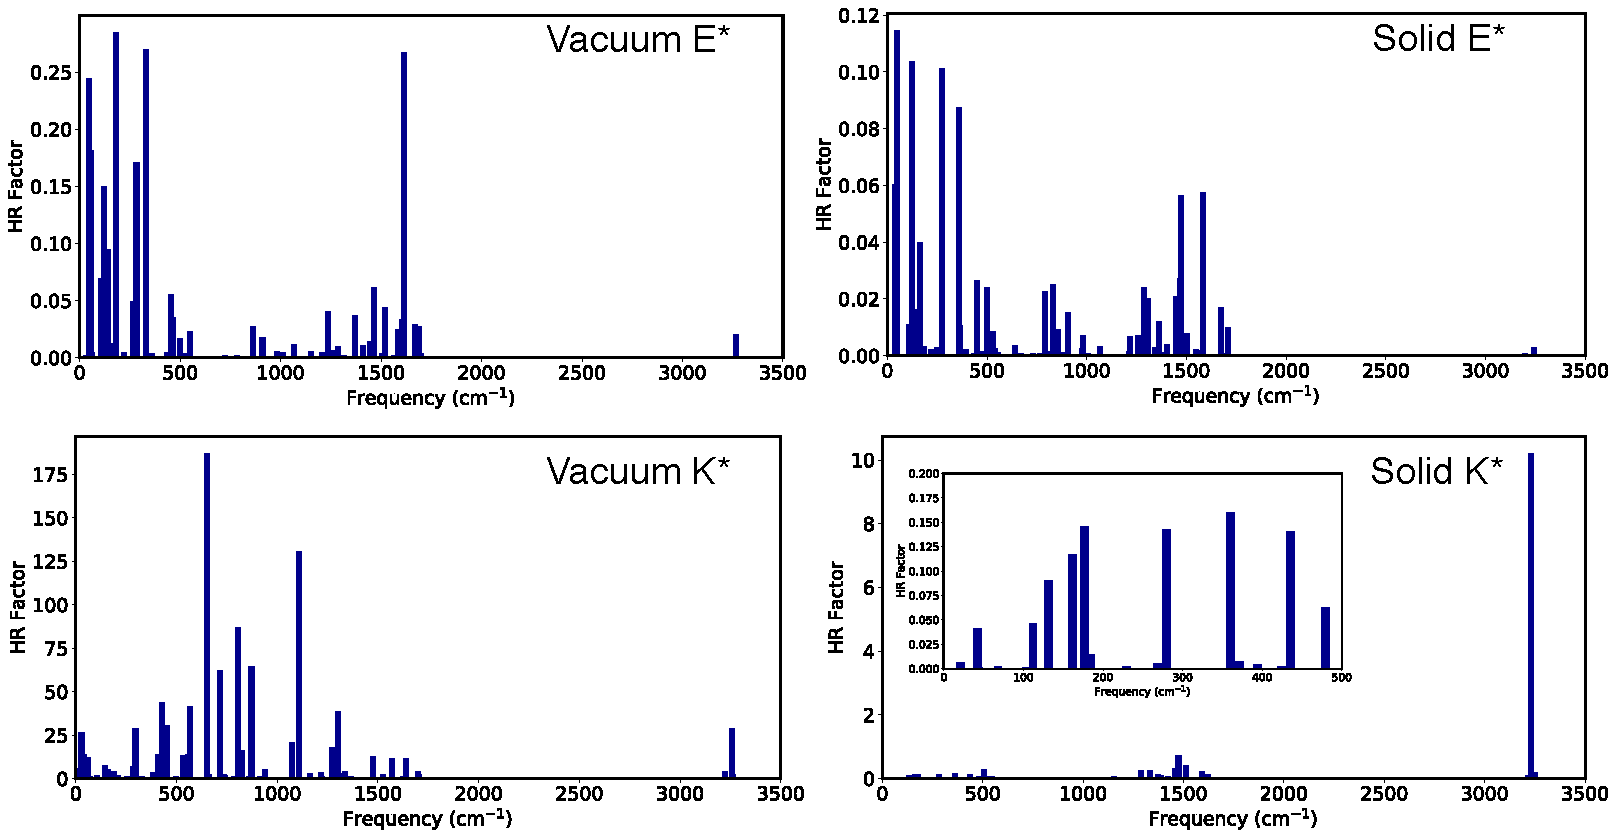
\includegraphics[width=\linewidth]{5ConnectingCrystalStructure/HC1_DUSHIN}
  \caption[HR factors for \textbf{HC1}]{Huang-Rhys factors associated with each normal mode calculated \textit{via} the Duschinsky rotation matrix between the E* and \szero{}, and K* and \szero{} electronic states for \textbf{HC1}. Frequencies 0-500 cm\textsuperscript{-1} in the solid state are shown in the inset.}
  \label{figure: HC1_DUSHIN}
\end{figure}

\begin{figure}[H]
\centering
  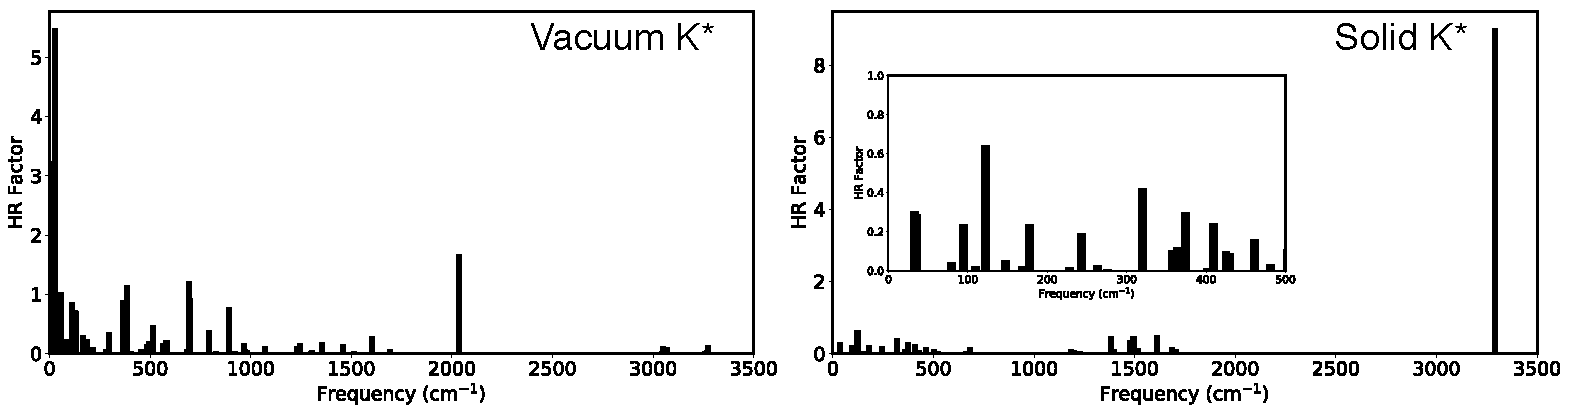
\includegraphics[width=\linewidth]{5ConnectingCrystalStructure/HC5_DUSHIN}
  \caption[HR factors for \textbf{HC5}]{Huang-Rhys factors associated with each normal mode calculated \textit{via} the Duschinsky rotation matrix between  K* and \szero{} electronic states for \textbf{HC5}. Frequencies 0-500 cm\textsuperscript{-1} in the solid state are shown in the inset.}
  \label{figure: HC5_DUSHIN}
\end{figure}

\begin{figure}[t]
\centering
  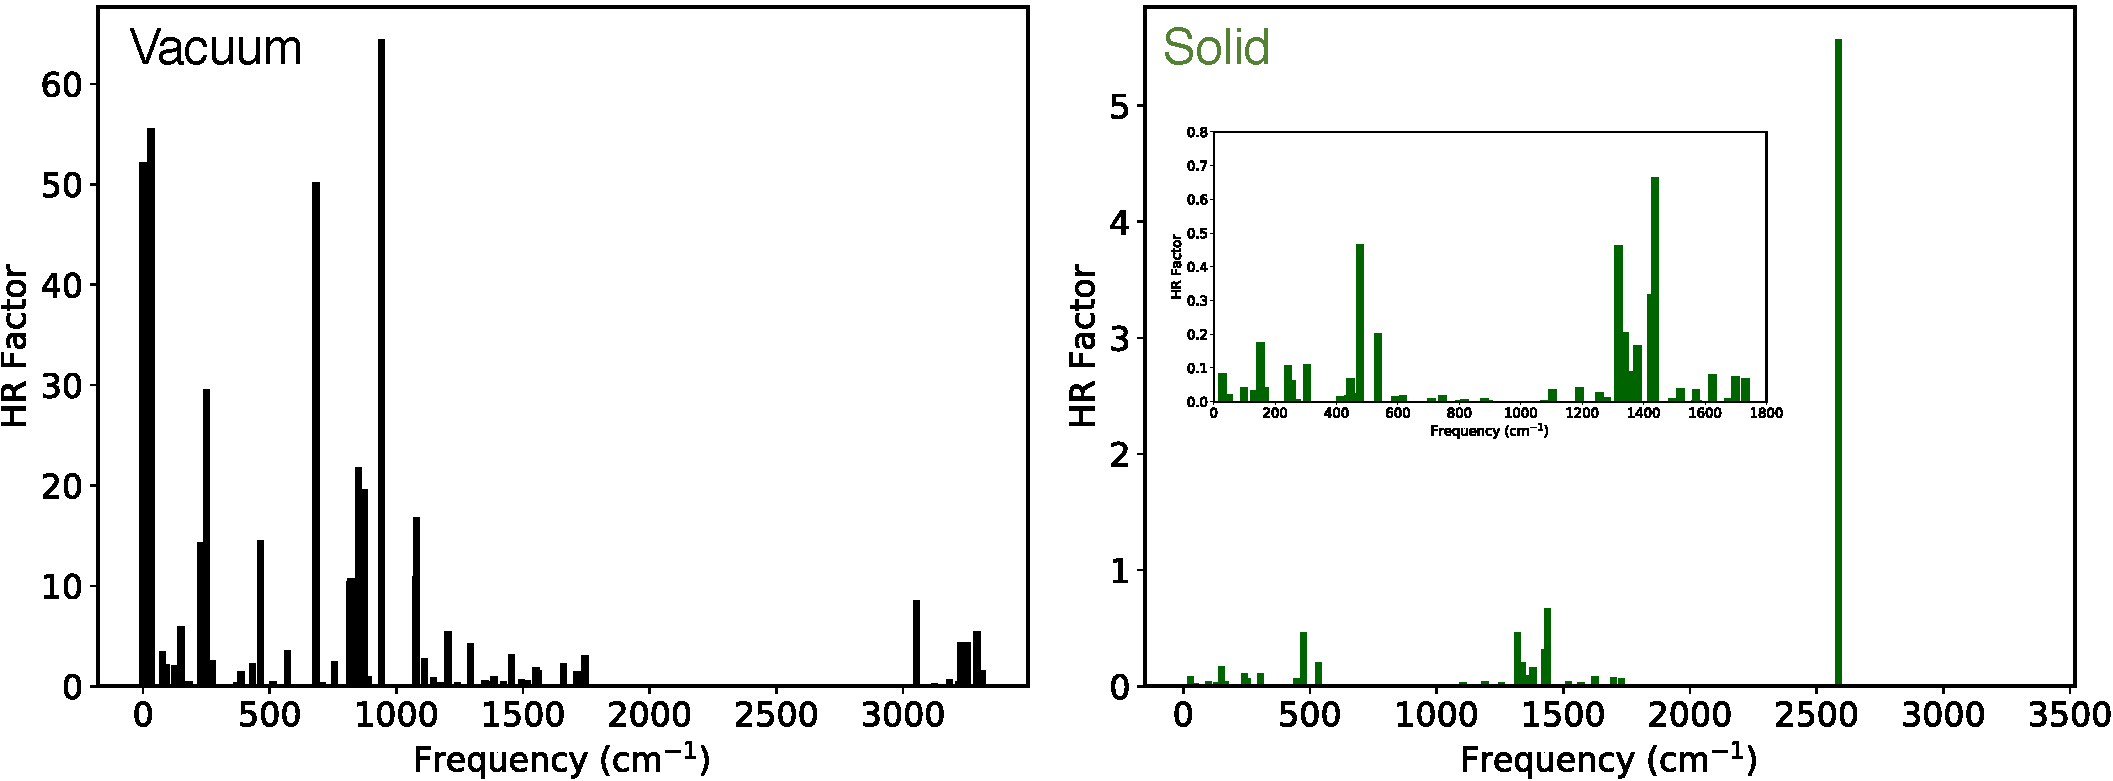
\includegraphics[width=\linewidth]{5ConnectingCrystalStructure/HP1_DUSHIN}
  \caption[HR factors for \textbf{HP1}]{Huang-Rhys factors associated with each normal mode calculated \textit{via} the Duschinsky rotation matrix between K* and \szero{} electronic states for \textbf{HP1}. Frequencies 0-500 cm\textsuperscript{-1} in the solid state are shown in the inset.}
  \label{figure: HP1_DUSHIN}
\end{figure}

In \textbf{HC5} there is no stable E* minimum in either vacuum or the solid state for the monomer chromophore. In vacuum, the HR factors are much less than in \textbf{HC1} due to the rotation angle at the minimum being less distorted. The molecule is more planar and is closer in structure and vibrational signature. At larger rotation angles the MECI is reached. HR factors are reduced in the solid state, in particular for the rotational modes, but with the O-H stretch HR factor increasing.   %Here the OH stretch is at 2036 cm\textsuperscript{-1}. In the molecular crystal the OH-

For \textbf{HP1}, large reorganisation energies, and correspondingly large HR-factors, are associated with low-frequency rotational modes. Indeed, such is the displacement between modes in the ground and excited states, the total reorganisation energy is 41 eV, whereas the adiabatic value 3.89 eV. As such, the harmonic approximation is invalid here due to the excited state potential energy surface anharmonicity. In the solid state, the normal modes associated with rotation are significantly reduced, whilst the largest HR factor is associated with the stretching of the phenol oxygen. This is to be expected, since it is along this coordinate that ESIPT occurs, and hence is has the largest HR-factor. In solid state, $\lambda_{NM}$ is 2.19 eV, compared with $\lambda_{A}$ of 1.24 eV.  

In the case of the \textbf{HC} and \textbf{HP} systems, the AIE behaviour can not be directly attributed to the reduction of the HR factors in the solid state compared to vacuum. Such is the complexity of the PES, where ESIPT and rotation occur in the excited state (in vacuum), the surfaces are highly anharmonic and the validity of the \ac{FGR-RIM} scheme is not clear. As such, it is not the focus of our investigation into the AIE behaviour of these systems.

%%%%%%%%%%%%%%%%%
\subsection{Analysis of Crystal Packing} \label{section: Connecting_Motifs}
%%%%%%%%%
%%%%%%%%%
In this section we use several techniques to analyse the crystal structures of the eleven compounds of Table \ref{table: chalcones}. The crystalline environment of each crystal is examined initially from the perspective of a monomeric chromophore. To this end, we use Voronoi cell volumes $V_{cell}$ and van der Waals volumes $V_{vdW}$ to determine a Voronoi index $V_{i}=V_{cell}/V_{vdW}$, a metric indicating the normalised accessible volume for a monomer in the crystal. $V_{i}$ values (Figure \ref{figure: voronoi_index}) range from 1.29-1.48, showing that despite the substituent and packing differences, the each monomer in the system has between 30\%-50\% of its van der Waals volume to freely vibrate, rotate or translate. For the \textbf{HC} systems, the average $V_{i}$ is 1.36$\pm$0.06, and 1.30$\pm$0.01 for the \textbf{HP} systems. The accessible volume for the \textbf{HC} systems shows greater variation but is overall slightly higher than for the less varied \textbf{HP} systems. The increased volume for the \textbf{HC} systems theoretically allow for greater nuclear relaxation in the excited state. However, reorganisation eneergies (Section \ref{section: Connecting_Marcus}) for the \textbf{HP} systems are larger than for \textbf{HC}, showing the importance of the electronic effects over geometric considerations. 

Exciton transport has been shown to occur through coherent or incoherent hopping between molecular sites, and thus it is important to understand the possible intermolecular transport channels in the \textbf{HC} and \textbf{HP} systems. To determine the intermolecular relationships, we examine the topology of the molecular crystals of \textbf{HC} and \textbf{HP} families by considering dimer configurations. Crystal morphologies are commonly described qualitatively as herringbone, face-face, edge-tail, \textit{etc}. Here we take a more of quantitative approach by constructing maps of each crystal, based on a geometric description of the dimers. These maps allow the topology of the crystal to be analysed graphically.
\begin{figure}[t]
\centering
  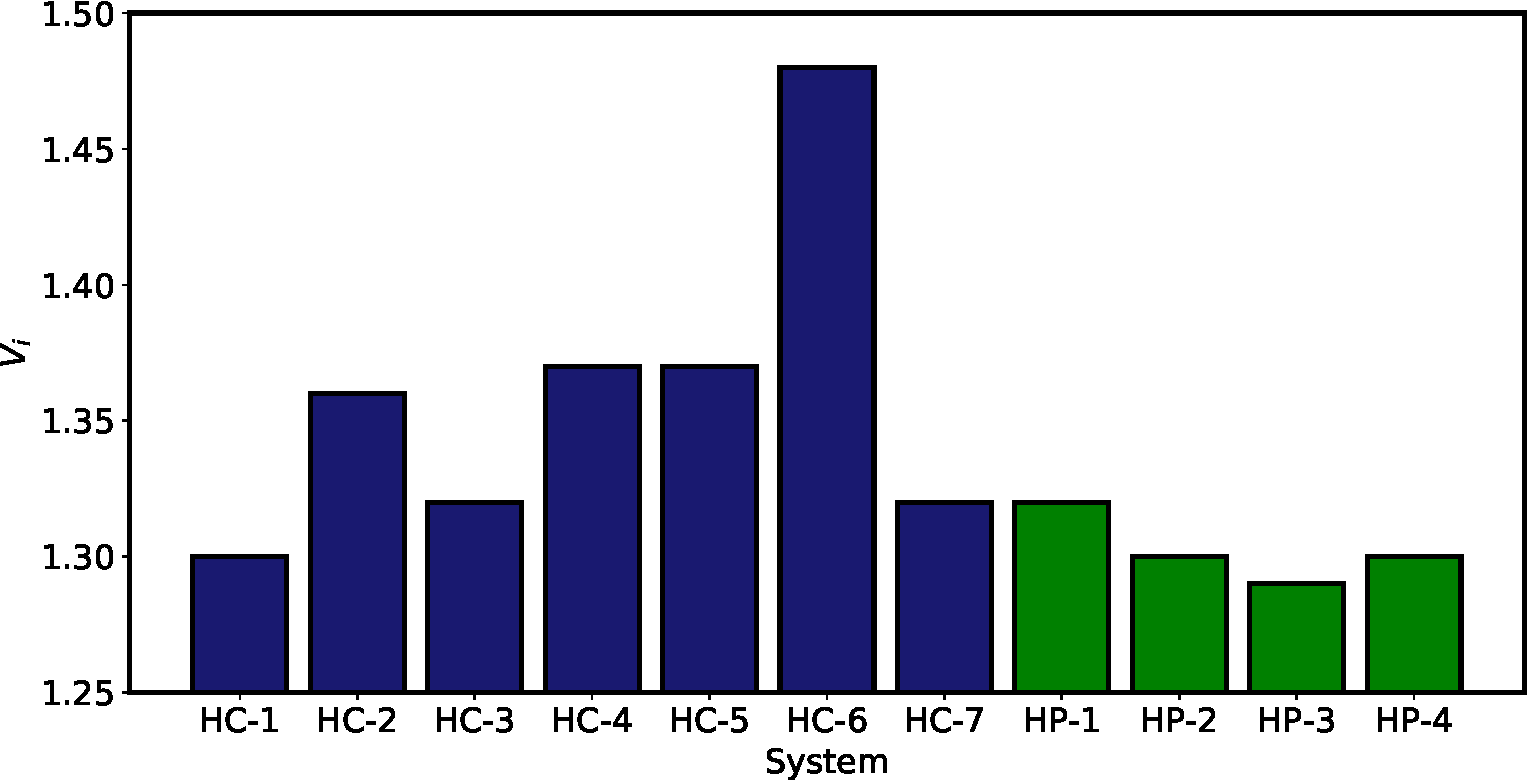
\includegraphics[width=0.8\linewidth]{5ConnectingCrystalStructure/Voronoi_Index}
  \caption{Voronoi indices for \textbf{HC} and \textbf{HP} crystal structures.}
  \label{figure: voronoi_index}
\end{figure}

Dimers are quantified through three angle variables, $\alpha$, $\beta$, and $\gamma$. These are depicted in Figure \ref{figure: dimer_schematic_alpha}, and example dimers with associated angles are given in Figure \ref{figure: motif_examples}. Three axes, $x$, $y$, $z$, are defined on each molecule $i$ and $j$ of the dimer, where $x$ and $y$ are the long and short axes of the molecule, and $z$ is the orthogonal vector. These vectors comprise an orthogonal basis to describe the dimer. The angles are then defined as:
\begin{itemize}
\item[$\bullet$] $\alpha$: The azimuthal angle between the monomers shown as the black angle in Figure \ref{figure: dimer_schematic_alpha}. Calculated as the angle between the $z$-axis located at the centroid of monomer $i$, and the vector connecting two centroids. $\alpha$ is calculated twice, once with each monomer as the reference. The smallest angle is chosen, such that 0\degree{}$\leq\alpha\leq{}90\degree{}$.

\item[$\bullet$] $\beta$: The angle between the two short-axis vectors $y$ of each molecule, shown in green in Figure \ref{figure: dimer_schematic_alpha}. $\beta$ ranges from 0\degree{} to 180\degree{}, tracking whether monomers are aligned cofacially parallel ($\beta=$0\degree{}, CoF-P), or cofacially antiparallel ($\beta=$180\degree{}, CoF-A), or in a herringbone edge-face manner (90\degree{}, Hb), and all configurations in between. $\beta$ is commonly described as the ``herringbone'' angle. 

\item[$\bullet$] $\gamma$: The angle between the long-axis vectors $x$, ranging from 0\degree{} (parallel, P) to 180\degree{} (antiparallel, A). At $y=$ 90\degree{}, the dimer is T- or L-shaped, dependent on the $x$-slip. 
\end{itemize}

\begin{figure}[t]
\centering
  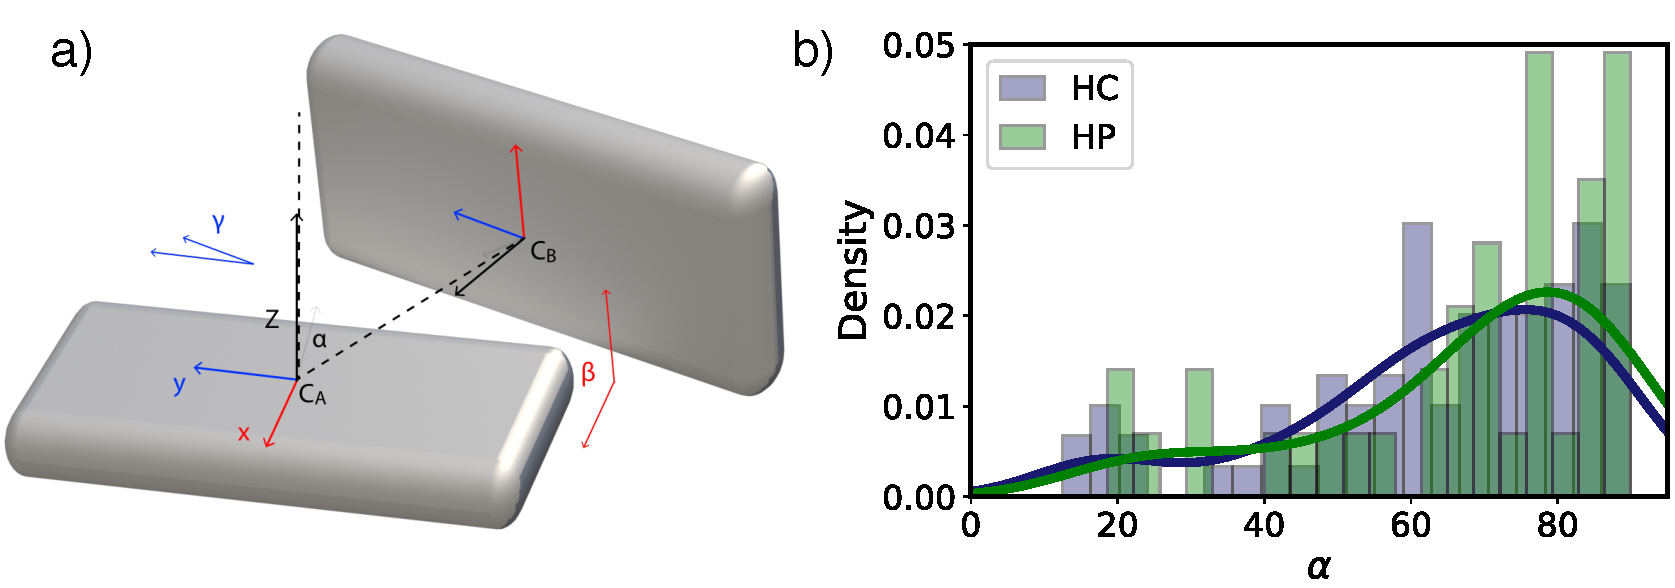
\includegraphics[width=0.8\linewidth]{5ConnectingCrystalStructure/dimer_schematic_alpha}
  \caption[Schematic of $\alpha$, $\beta$, and $\gamma$ angles for classification of dimers.]{Panel a), left; schematic of two monomers, and the $\alpha$, $\beta$, and $\gamma$ angles used to classify dimer configurations. Panel b), right; distribution of $\alpha$ angles for dimers in \textbf{HC} and \textbf{HP} systems.}
  \label{figure: dimer_schematic_alpha}
\end{figure}

\begin{figure}[t]
\centering
  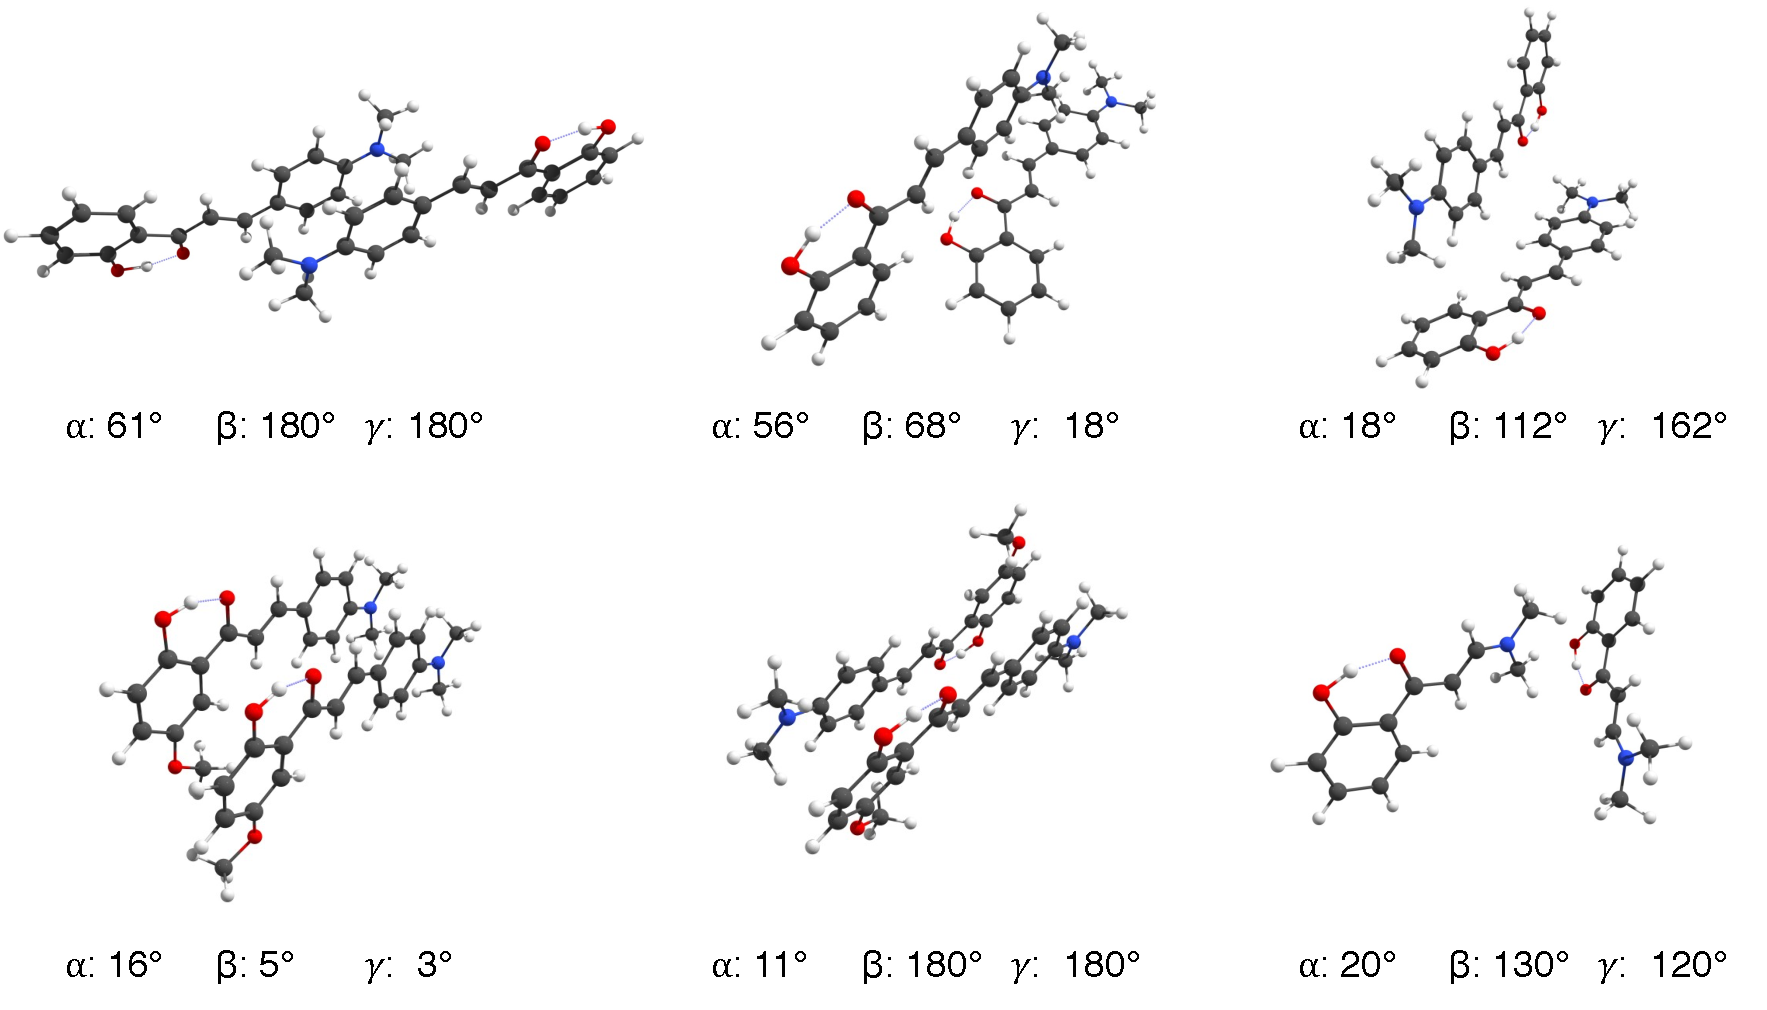
\includegraphics[width=0.9\linewidth]{5ConnectingCrystalStructure/motif_examples}
  \caption[Example dimers in \textbf{HC1}, \textbf{HC5}, and \textbf{HP1}.]{Example dimers and associated $\alpha$, $\beta$ and $\gamma$ angles in \textbf{HC1}, \textbf{HC5}, and \textbf{HP1}.}
  \label{figure: motif_examples}
\end{figure}

In Figure \ref{figure: dimer_schematic_alpha}b the distribution density of the $\alpha$ angle is shown for the cofacially stacked \textbf{HC} and \textbf{HP} systems. The distribution is heavily skewed towards 90\degree, indicating that for the majority of cofacial dimers, there is little overlap between the centroids of the monomers. As such, it can be expected that in each molecular crystal there are few dimers with the configuration required for efficient charge or energy transfer, and that transfer will occur through only a few particular dimers. 
\begin{figure}[t]
\centering
  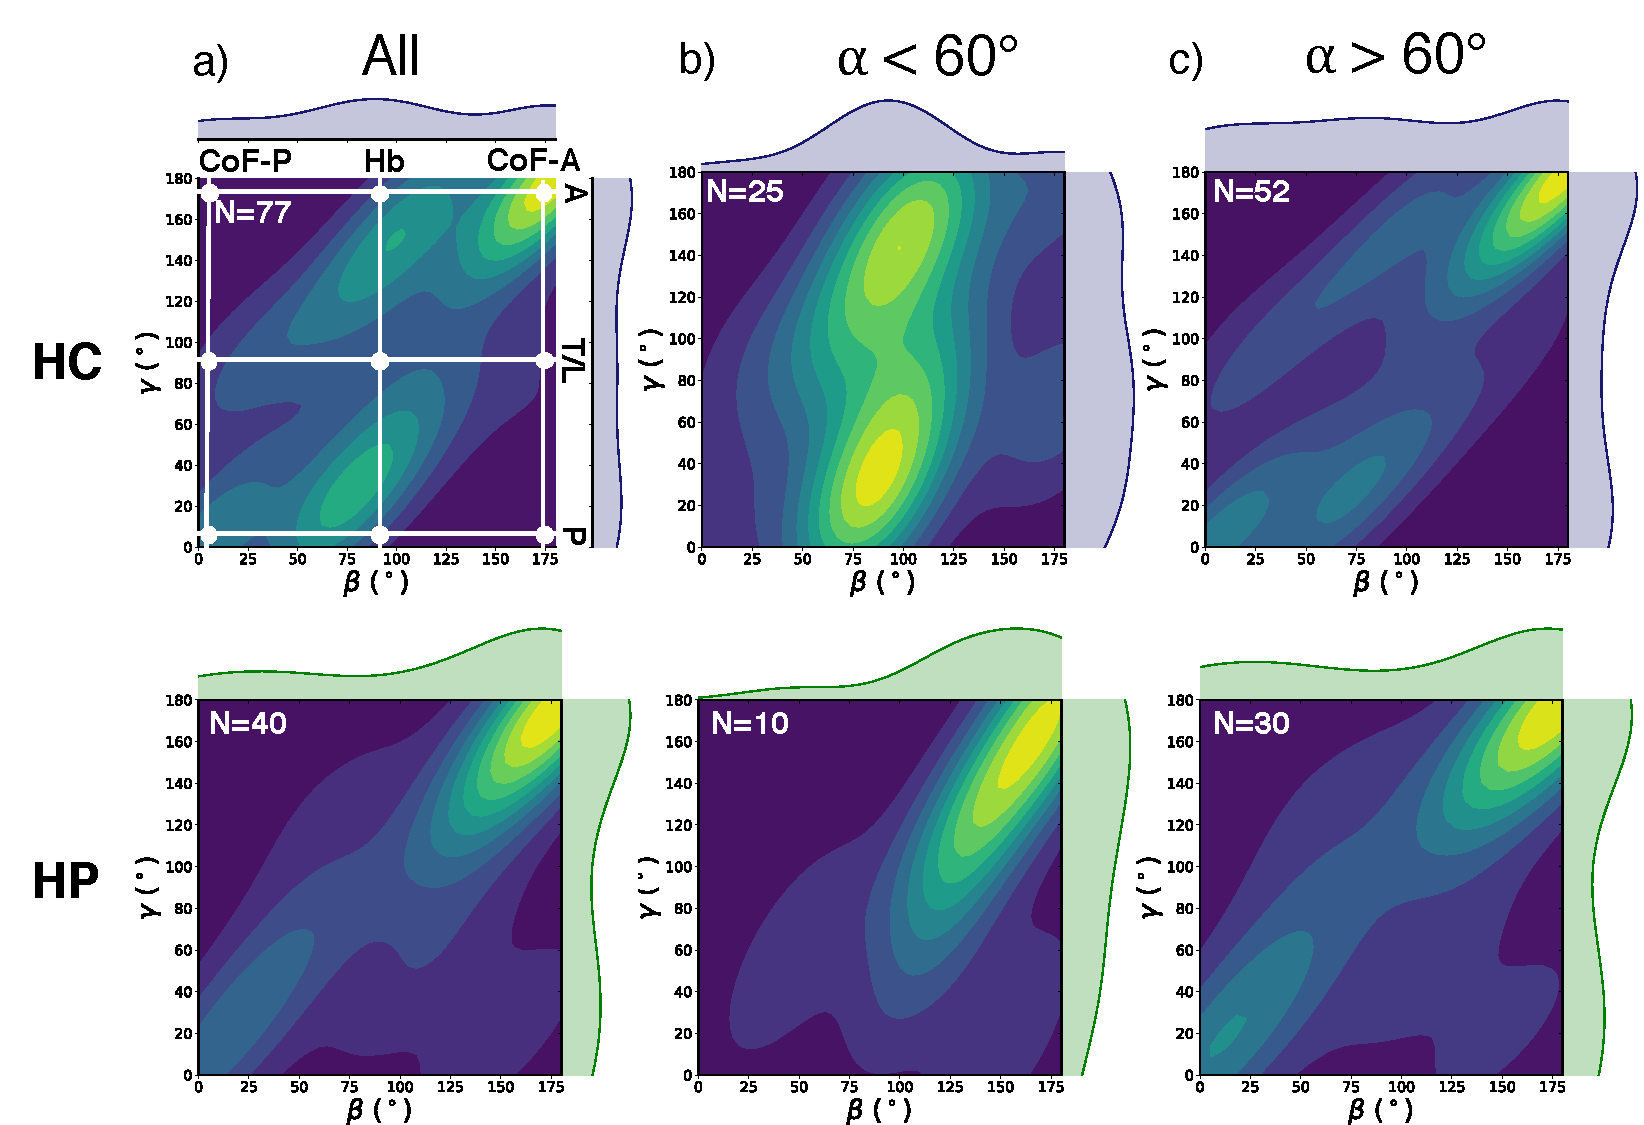
\includegraphics[width=0.9\linewidth]{5ConnectingCrystalStructure/dimer_classification}
  \caption[Probability density maps of $\beta$ and $\gamma$ angles.]{Panel a), left; Probability density map of the $\beta$ and $\gamma$ angles for \textbf{HC} (top) and \textbf{HP} (bottom) dimers. Key configurations are labelled on the axes, as explained in the text. Panel b), centre; probability density for the subset of dimers where $\alpha$ \textless{}  60\degree{}.  Panel c), right; probability density for the subset of dimers where $\alpha$ \textgreater{} 60\degree{}.}
  \label{figure: dimer_classification}
\end{figure}

Figure \ref{figure: dimer_classification} shows the dimer distribution densities for the $\beta$ and $\gamma$ angles for \textbf{HC} (top row) and \textbf{HP} (bottom row). Key regions are highlighted as an example in the upper plot of panel a); for example at $\beta$=90,$\gamma$=0, a herringbone (Hb) stack is witnessed with the long axes arranged in parallel. For both \textbf{HC} and \textbf{HP} systems, the majority of dimers have $\beta$ and $\gamma$ angles close to 180\degree{} (top right of plot), indicating that the most common dimer configuration is a cofacial arrangement where the carbonyl groups align antiparallel, at opposing ends of the molecule from eachother. This results in an antiparallel alignment of the \sone{} transition dipole moment of each monomer.  However, as panels b) and c) show, when the $\alpha$ angle is used as a filter, the configurations with more acute azimuthal angles are mostly herringbone in nature for \textbf{HC}, with carbonyl groups at the same ($\gamma=$0\degree) or opposite ends of the dimer ($\gamma=180\degree$). There also exist dimers close to this arrangement, with deviations in both $x$ and $y$. In the relatively few \textbf{HP} systems with  $\alpha$\textless{60}\degree{}, configurations lie on the diagonal between herringbone and cofacial.

The cofacial arrangements favoured by the Kasha model occur at large slip displacements in the $x$ or $y$  plane ($\alpha$\textgreater{60}), and are more like edge-edge coplanar arrangements rather than the well-known $\pi$-stack. Only in \textbf{HC5} is there significant cofacial $\pi$-stacking between dimers, with other cofacial arrangements in \textbf{HC} and \textbf{HP} having larger $x$-slip, as is common for aromatic groups. For \textbf{HC} compounds, 63\% of the cofacially aligned dimers have a $x$-slip of less than half a molecule, whereas 68\% of cofacially-algined \textbf{HP} dimers have a $x$-slip of more than half a molecule, as shown in Figure \ref{figure: xslip_density}. So while the cofacial, $\pi$-stacked arrangement is rare for both families, it is more prominent in \textbf{HC} compounds than their mono-aryl \textbf{HP} counterparts. The cofacial arrangement is particularly dominant in \textbf{HC5}.


\begin{figure}[t]
\centering
  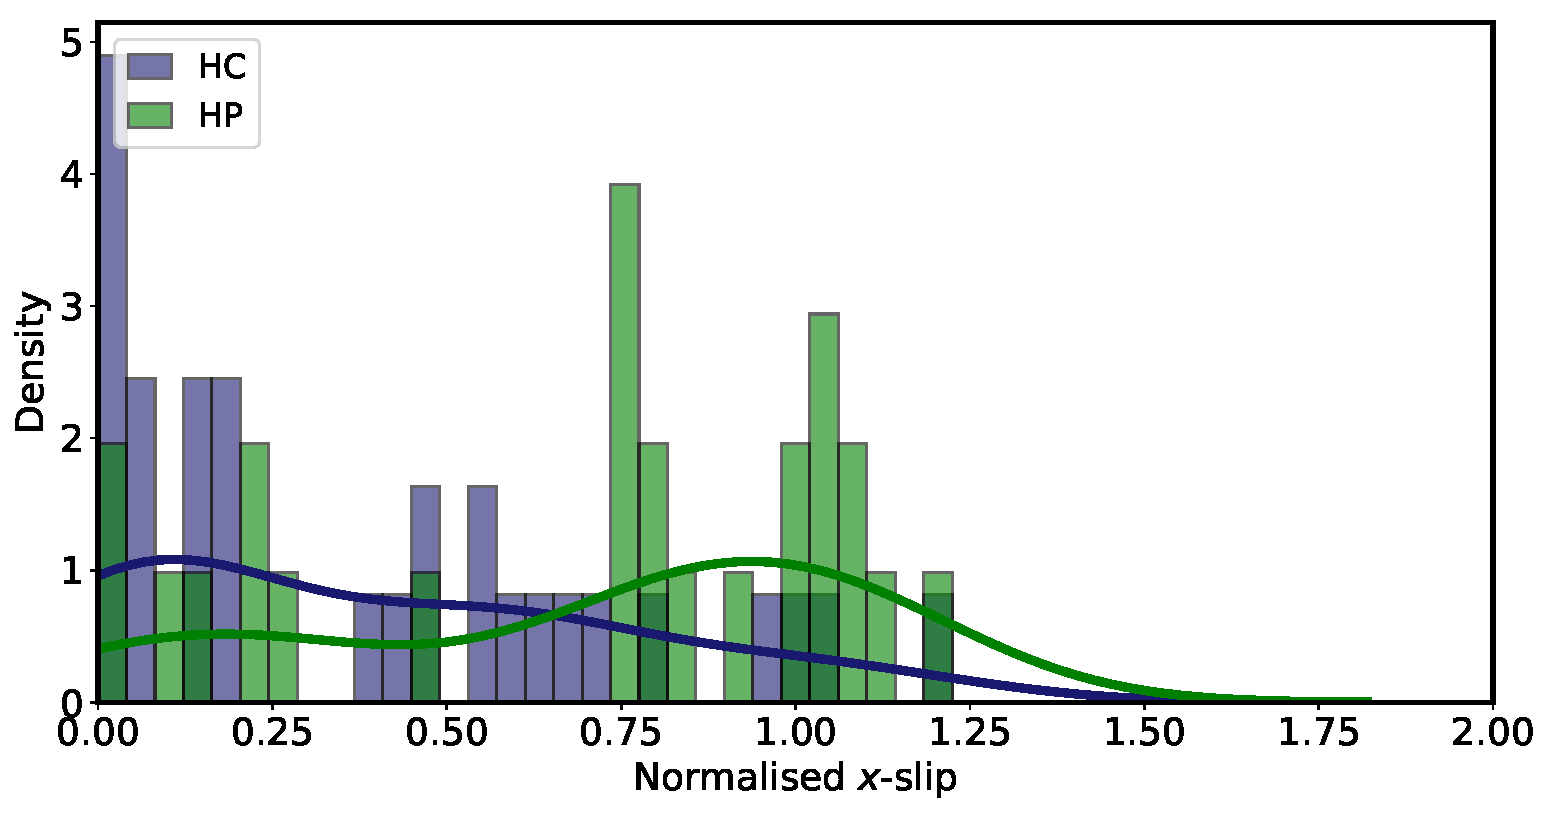
\includegraphics[width=0.8\linewidth]{5ConnectingCrystalStructure/xslip_density}
  \caption[$x$-slip densities for dimer configurations of \textbf{HC} and \textbf{HP} systems]{The density of slip distances for each molecular dimer in the $x$-plane (long axis) for cofacial dimers. The slip is normalised by the length of the long axis $x$ for each molecule, such that slip is molecule independent.}
  \label{figure: xslip_density}
\end{figure}

Overall, the significant dimer arrangement in \textbf{HP} compounds is a herringbone structure, with the majority of cofacial arrangements having a large $x$ or $x$-slip with minimal $\pi\pi$ interactions due to the single aryl groups aligning at $y$=180\degree. The $\alpha$ angle is generally larger than in \textbf{HC}, indicating a larger slip, with overlapping monomers distributed around a cofacial stacking. The prominence of the herringbone arrangement in \textbf{HC} systems is replaced by a propensity for a T-shape packing, quantified by the $\gamma$ angles distributed around 90\degree. In the next section, we show how these geometric parameters influence the exciton coupling in the \textbf{HC} and \textbf{HP} families.

\subsection{Intermolecular Interactions in the Molecular Crystal}\label{section: Connecting_Interactions}

Localisation of the electronic excited state onto one monomer of the molecular crystal has been shown to be an important step in the relaxation process of ESIPT systems in the solid state in Chapter \ref{chapter: Inter}. For the dimers discussed above, the coupling $J_{ij}$ between monomers $i$ and $j$ is calculated in Troisi's diabatization scheme based on the orthogonal transformation of adiabatic states to diabatic states (Equation \ref{equation: diabatic matrix}).\cite{Arago2015,Fornari2016}. In this Chapter this method is extended to asses the effect of a third monomer $k$ on the exciton coupling, where in a trimer chromophore, $\textbf{H}^D$ becomes a 3x3 matrix
\begin{equation}
\small
\label{equation: 3x3 diabatic matrix}
\begin{bmatrix}
E_{i}^D & J_{ij} & J_{ik}\\
J_{ji} & E_{j}^D & J_{jk} \\
J_{ki} & J_{kj}& E_{k}^D
\end{bmatrix}
=
\begin{bmatrix}
C_{11} & C_{12} & C_{13}\\
C_{21} & C_{22} & C_{23}\\
C_{31} & C_{32} & C_{33}
\end{bmatrix}
\begin{bmatrix}
E_{i}^A & 0 & 0\\
0 & E_{j}^A & 0\\
0 & 0 & E_{k}^A\\
\end{bmatrix}
\begin{bmatrix}
C_{11} & C_{12} & C_{13}\\
C_{21} & C_{22} & C_{23}\\
C_{31} & C_{32} & C_{33}
\end{bmatrix}
\end{equation} 
where the coupling $J_{ij}$ between monomers $i$ and $j$ incorporates the effect of monomer $k$, which can quantified through comparison of the dimeric and trimeric $J_{ij}$. Analysis of excitations at the Franck-Condon geometry for a trimer chromophore show that for \textbf{HP1}, the bright state is delocalised over two of the molecules arranged in a cofacial arrangement. This is shown in Figure \ref{figure: trimer_excitations}. A delocalised state over the whole trimer is not observed. Analysis of the excitations of the three types of dimer inherent in the trimer reveal that in each case, regardless of the stacking arrangement and despite the close aggregation of monomers, the excitation is delocalised over no more than two monomers. 

\begin{figure}[t]
\centering
  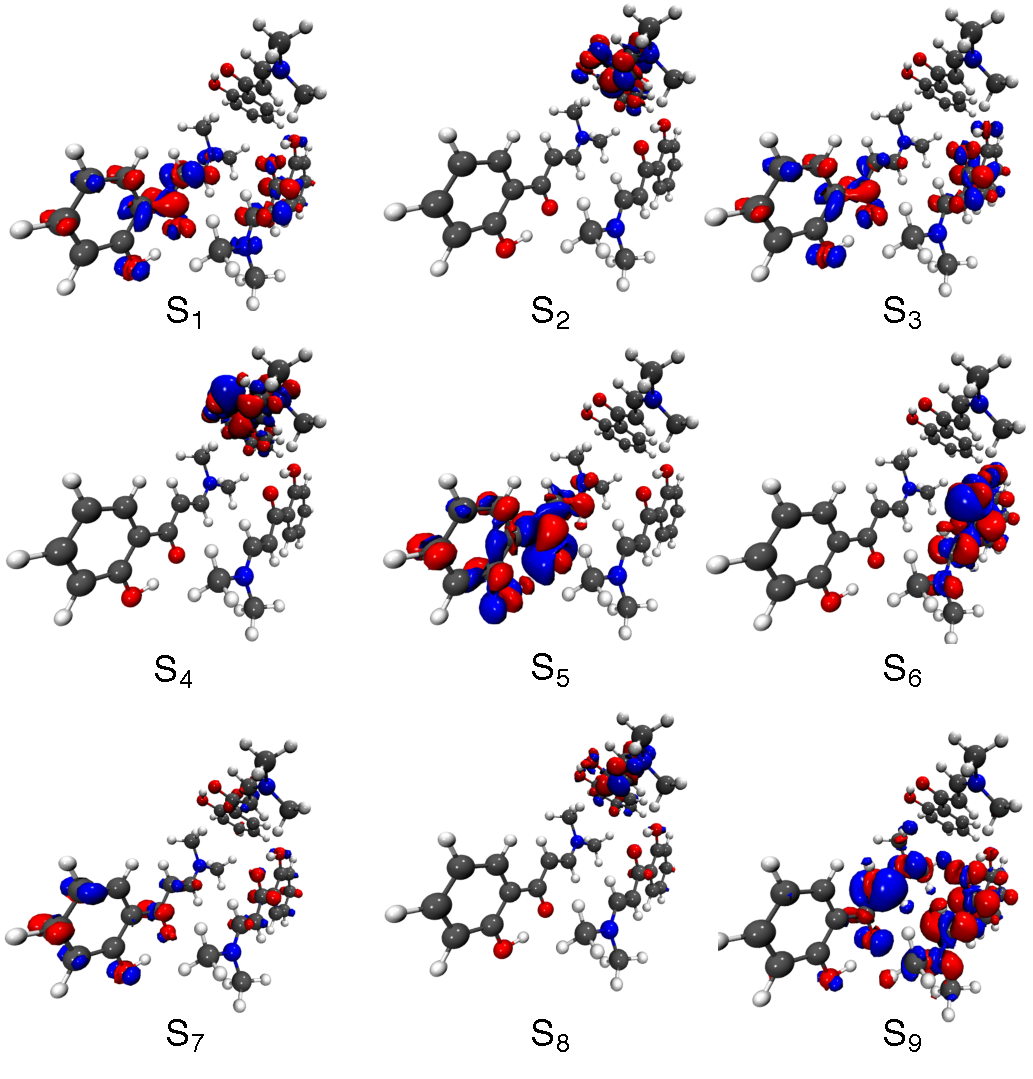
\includegraphics[width=0.8\linewidth]{5ConnectingCrystalStructure/trimer_excitations}
  \caption[Electron density diffrence maps for the first nine excited state of the \textbf{HP1} trimer.]{Electron density diffrence maps for the first nine excited state of the \textbf{HP1} trimer. The same colour scheme is used as in Figure \ref{figure: HC_Vac_Densities}}
  \label{figure: trimer_excitations}
\end{figure} 

To quantify the effect of the third molecule on the exciton coupling, the exciton coupling for a trimer system was calculated in \textbf{HP1}, \textbf{HC1}, and \textbf{HC5}. It is found that the addition of a third molecule has only a small effect on the dimer coupling in \textbf{HP1} and \textbf{HC1}, where the increased coupling in one dimer is compensated for by the decreased coupling in the other dimer, with difference of less that 0.02 eV. The largest effect is seen in \textbf{HC5} due to the cofacial packing of the trimer system, where the central monomer is sandwiched by two cofacially stacked monomers, one parallel and one antiparallel, as shown in \ref{figure: trimer_couplings}. For \textbf{HC1}, two trimers are used to capture both parallel and antiparallel stacked dimers. 

These perturbations are no larger than the inherent modulation of couplings in the dynamic regime.\cite{Arago2015,Arago2016} As such, focus from here will be on dimer couplings where the presence of exterior molecules has been neglected. The exciton couplings for all dimers and the identity of the dimer with the largest $J$ are shown in Figure \ref{figure: couplings}. 
\begin{figure}[t]
\centering
  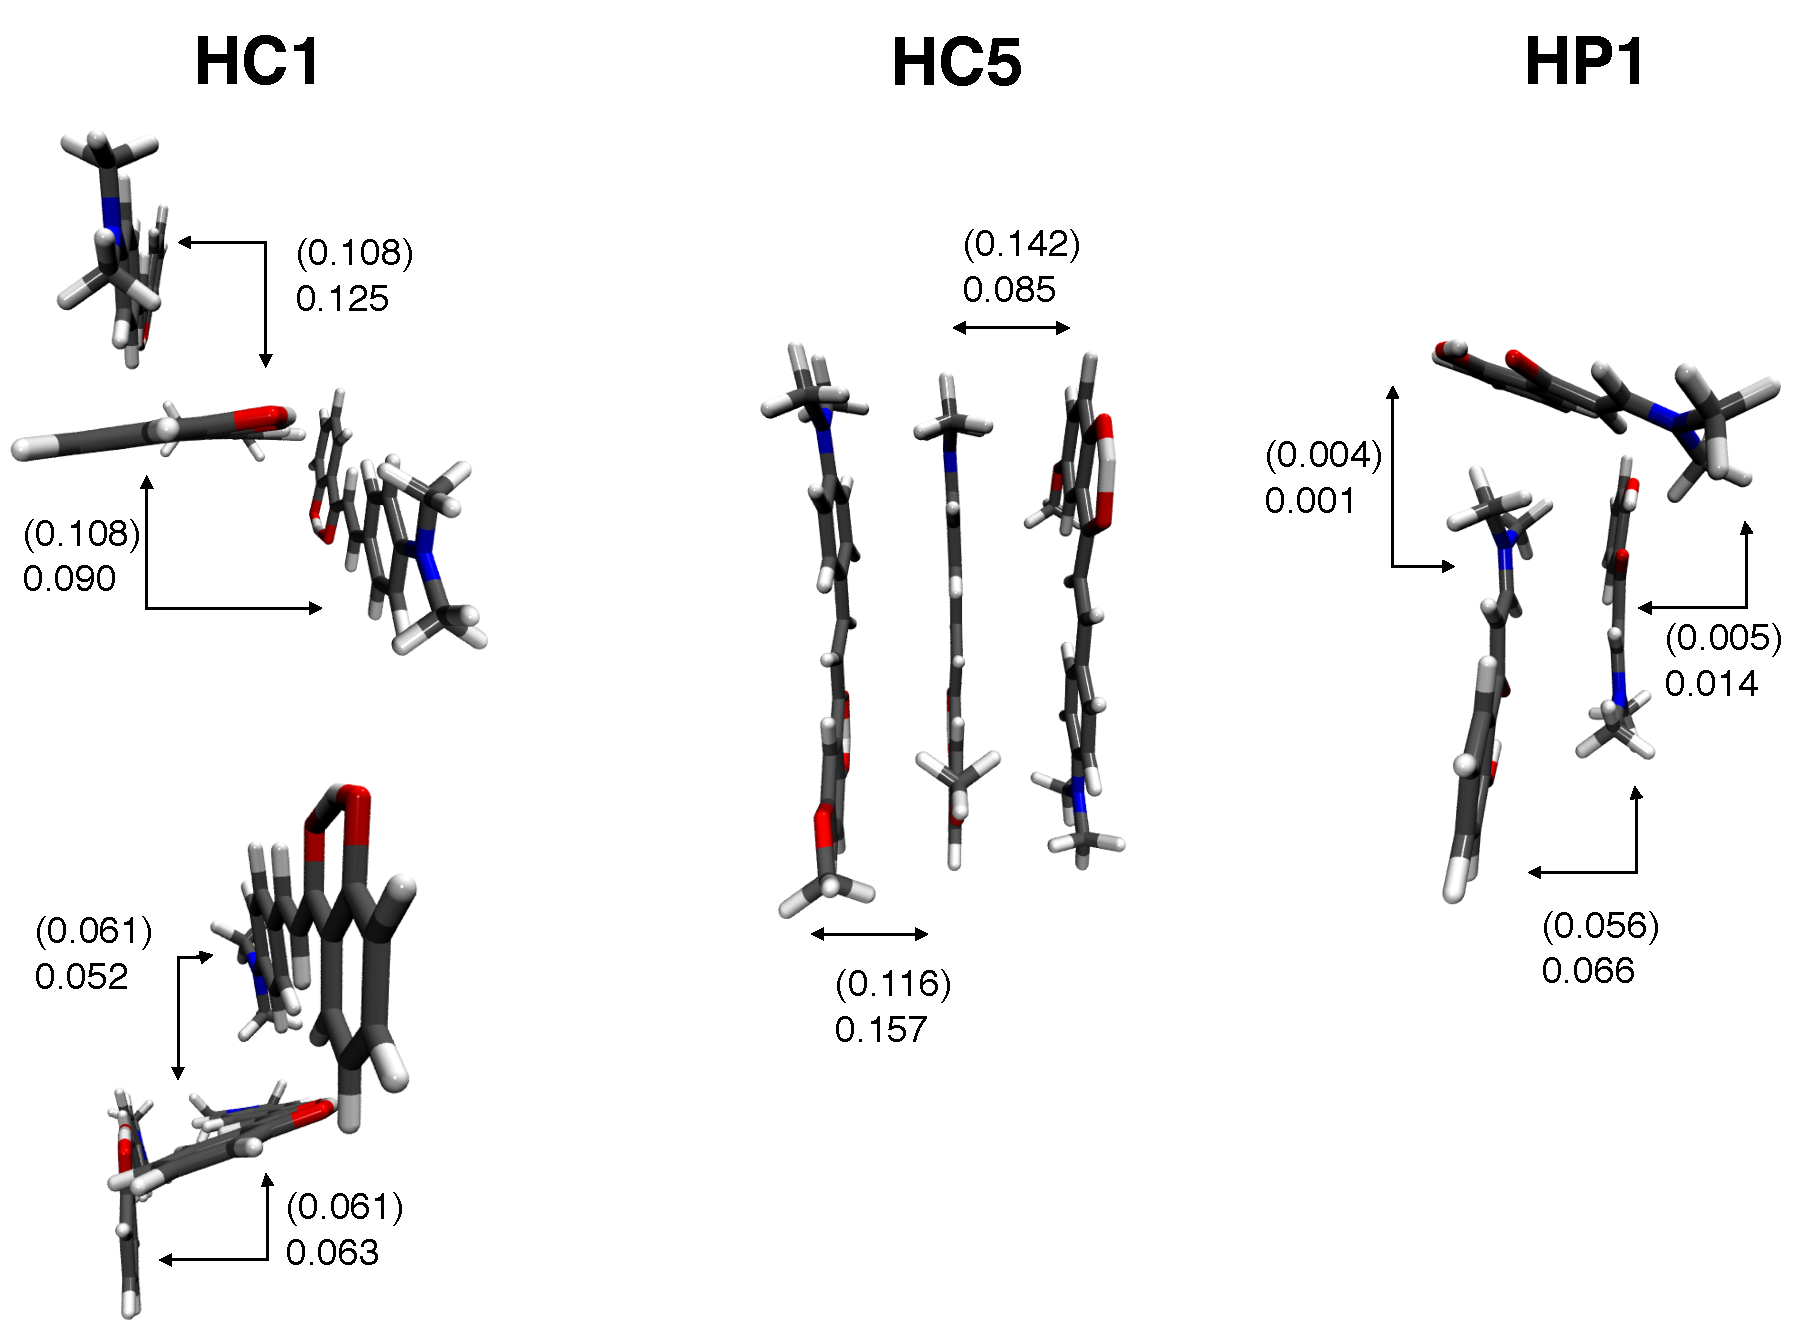
\includegraphics[width=0.8\linewidth]{5ConnectingCrystalStructure/trimer_couplings}
  \caption[Trimer exciton couplings]{Schematic of the trimers extracted from unit cells of \textbf{HC1}, \textbf{HC5} and \textbf{HP1}. Exciton couplings considering the trimer are shown. In parenthesis are the couplings considering only a dimer. Calculated at $\omega$B97X-D/6-311++G(d,p) level of theory.}
  \label{figure: trimer_couplings}
\end{figure}


\begin{figure}[t]
\centering
  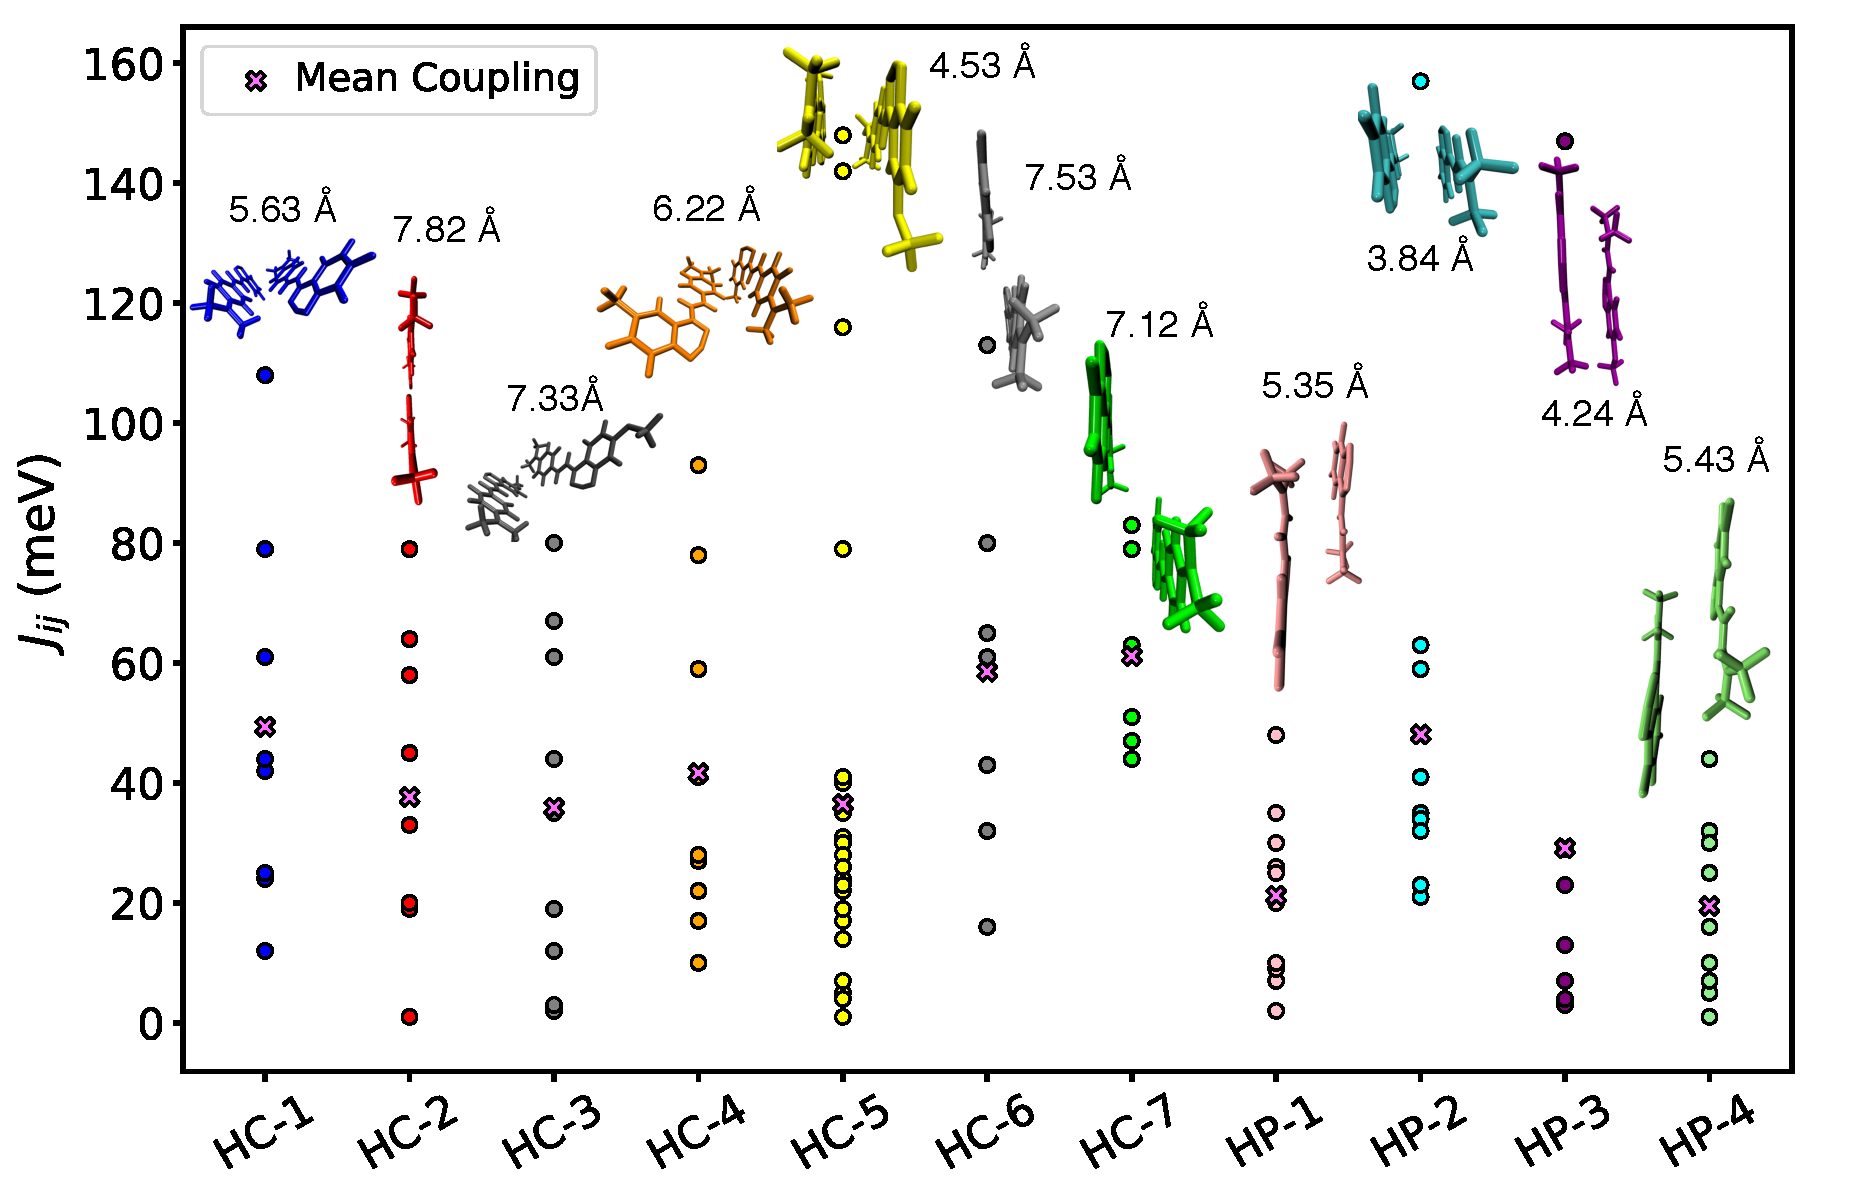
\includegraphics[width=0.9\linewidth]{5ConnectingCrystalStructure/couplings}
  \caption[Exciton couplings in \textbf{HC} and \textbf{HP} systems]{Exciton couplings $J$ between monomers $i$ and $j$ in the dimers identified in \textbf{HC} and \textbf{HP}. The mean coupling is also shown, along with the distance in angstroms between the constituent monomer centroids.}
  \label{figure: couplings}
\end{figure}

In \textbf{HC1-4}, where the closest packed dimers are herringbone in nature, similar dimer configurations are present. For \textbf{HC-2}, the identity of the dimer with the largest coupling changes due to a lateral displacement of one monomer increasing the centroid distance to 8.5 {\AA} and thus reducing the coupling in the herringbone stacked dimer. The identity of the largest coupled dimer changes to a cofacial, edge-edge stacked dimer with $\alpha=87\degree$, where minimal overlap reduces the coupling $J$. For \textbf{HC-1,3,4}, the herringbone stacking pattern is exhibited where the largest coupling is found in \textbf{HC1}, where the monomers are most tightly packed. In \textbf{HC5-7}, face-face stacked dimers are more prevalent in the crystal structure. The size of the coupling in \textbf{HC6} is reduced compared to \textbf{HC5} due to the $y$ displacement of one the monomers. It is further reduced in \textbf{HC7} due to an increased $x$-slip. In the \textbf{HP} compounds, the large $\alpha$ and $x$-slip values systematically reduce the average coupling. In each \textbf{HP} derivative there exists one close packed, cofacial dimer which exhibits the largest coupling. In \textbf{HC2-3}, the crystal structures afford more efficient cofacial stacking with $x$-slip values of only 1{\AA}, resulting in the largest couplings of all investigated systems. 

As shown in  Figure \ref{figure: dimer_regressions}a, the coupling $J$ correlates linearly with half of the energy splitting for the \sone{} and \stwo{} states of the dimer. This is somewhat surprising, given the simplicity of the original model (Section \ref{section: lom intermolecular-interactions}), the polarity of the molecules in question and their generally nonparallel stacking. The energy splitting is perhaps the simplest way to obtain the exciton coupling in the Kasha regime, although it is more expensive than using atomic-centred transition charges, or the PDA approximation, since the supramolecular calculation must be done rather than one monomer calculation. At small intermolecular distances (\textless4{\AA}), these computationally efficient metrics can underestimate the couplings due to them only considering the Coulomb interaction.\cite{Kistler2013} The linear correlation here shows that the general Kasha interpretation of the coupling applies here and that the diabatization method to obtain the couplings reproduces the supramolecular coupling.

The role of H- and J-aggregates is investigated by assigning dimers based on the oscillator strength of the \sone{} (J) and \stwo{} (H) excitation, which offers better resolution than using the energy shift. This is summarised in Table \ref{table: dimer_types}.  In \textbf{HC}, systems, 60\% of dimers are J-aggregates, while in \textbf{HP} systems the J-aggregate population is 58\%. For \textbf{HC-4} and \textbf{HC-5}, which are nonemissive, the J-aggregate population drops to 22\% and 32\%, respectively. Important to note, however, is that emission in \Kstar{} is from a localised excited state, and thus monomer regime should dominate the emission characteristics. In ESIPT systems, the role of H- and J-agggregates is expected to be prominent only at absorption, and the J-aggregates are not responsible for the AIE behaviour due to the localised emission.

\begin{table}[t]
\centering
\caption[Dimer types for \textbf{HC} and \textbf{HP} molecular crystals]{Dimer types located for each molecular crystal. Significant increase in \textbf{HC5} dimers due to rotational flexibility of the methoxy group.} 
  \label{table: dimer_types}
  \begin{tabular}{cccc}
  \hline
  System & H-aggregates & J-aggregates & Total\\
  \hline
  \textbf{HC1} & 4 & 4 & 8\\
  \textbf{HC2} & 5 & 4 & 9 \\
  \textbf{HC3} & 4 & 5 & 9\\
  \textbf{HC4} & 7 & 2 & 9\\
  \textbf{HC5} & 19 & 10 & 29 \\
  \textbf{HC6} & 4 & 3 & 7\\
  \textbf{HC7} & 6 & 0 & 6\\
  \hline
  \textbf{HP1} & 5 & 5 & 10\\
  \textbf{HP2} & 5 & 6 & 11\\
  \textbf{HP3} & 4 & 5 & 9\\
  \textbf{HP4} & 5 & 5 & 10\\
  \hline
  \end{tabular}
\end{table}

In the Kasha model, for a perfectly stacked dimer with no $x$-slip, the oscillator strength of the \stwo{} state should be double that of the monomer state. Figure \ref{figure: dimer_regressions}b shows the relationship between the $x$-slip in the dimers and the oscillator strength, namely the difference in oscillator strength between the \stwo{} and \sone{} states in the dimer, normalised by the corresponding mononomer excitation energy. These systems generally fit the Kasha model, as when the $x$-slip is zero, the model predicts an enhanced \stwo{} intensity of 2.10 for the \textbf{HC}s and 1.83 for the \textbf{HP}s. With increasing $x$-slip, the difference in oscillator strength between the two states decreases until the inversion to J-aggregates is witnessed ($f_{S_{1}}>f_{S_{2}}$). For the \textbf{HC}s this occurs at a $x$-slip of 52\% and at 46\% for the \textbf{HC}s. The largest group of outliers are cofacially stacked dimers, where a larger shift is seen at lower slip distances due to the minimal $x$-slip and archetypal stacking.\cite{Gierschner2016} 
\begin{figure}[t]
\centering
  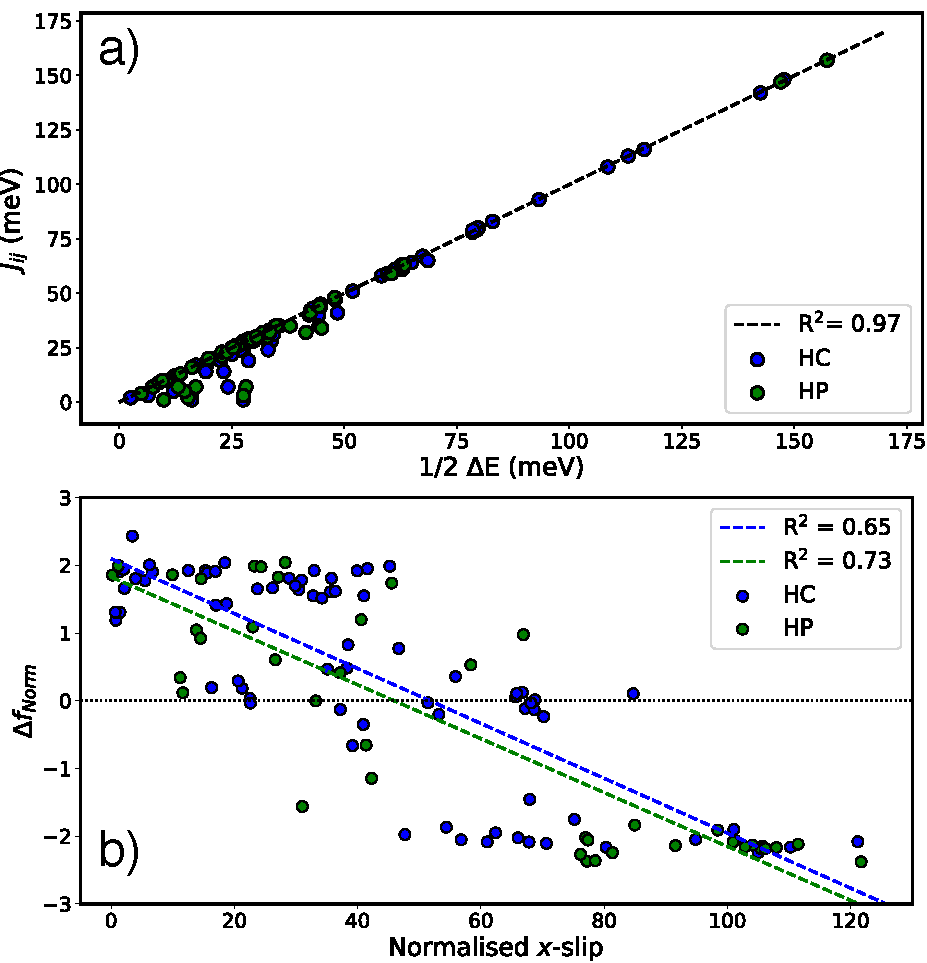
\includegraphics[width=0.8\linewidth]{5ConnectingCrystalStructure/dimer_regressions.pdf}
  \caption[Correlation between the energy splitting and exciton coupling]{Panel a), top; Correlation between the energy splitting of the dimer states and the exciton coupling. Panel b), bottom; Linear regression of the $x$-slip against the difference in oscillator strength between the \stwo{} and \sone{} states in dimers.}
  \label{figure: dimer_regressions}
\end{figure}



%%%%%%%%%%%%%%%%%%
%%%%%%%%%%%%%%%%%%
\subsection{Exciton Hopping}\label{section: Connecting_Marcus}
%%%%%%%%%%%%%%%%%%
%%%%%%%%%%%%%%%%%%
For fluorescence to occur from the K* state, the exciton must localise onto one monomer to enable ESIPT. In competition with this is exciton hopping, which will prevent localisation. Exciton hopping rates $\nu_{ij}$ between monomers $i$ and $j$ in a molecular crystal can be calculated based on a Marcus hopping scheme,\cite{Stehr2014,Bruckner2016,Kimura2000,Bredas2004} 
\begin{equation}
\nu_{ij}=\frac{J_{ij}^2}{\hbar}\sqrt{\frac{\pi}{\lambda k_{B}T}}\exp\bigg[-\frac{\lambda}{4k_{B}T}\bigg]
\label{equation: marcus}
\end{equation}
where $k_{B}$ is the Boltzmann constant, $\hbar$ is the reduced Planck
constant, T is the temperature (298K), and $\lambda$ is the reorganisation energy.

Solid state reorganisation energies $\lambda_{A}$ in keto and, when located, enol minima were calculated for ONIOM((TD-)$\omega$B97X-D/6-31G(d):UFF) models with a monomer chromophore using Equation \ref{equation: lambda}. Figure \ref{figure: marcus_scatter_vdw} shows the exciton coupling, reorganisation energy, and the associated exciton hopping rate (using a log scale) for each dimer. In Table \ref{table: reorgs_rates} the reorgansiation energies and largest rates in each channel are given. The hopping rate $\nu$ is ultrafast in the enol regime (\textbf{HC1-4,6,7}), where the planar conformation confers a relatively low reorganisation energy $\lambda$ (244 meV on average). The lowest $\nu$ for \textbf{HC1} is \SI{5e11}{s^{-1}}, while the rate of ESIPT in the molecular crystal, through time resolved spectroscopy, is \SI{3e11}{s^{-1}}.\cite{Zahid2017} In Section \ref{section: NRdecay_Dynamics}, it was calculated that the rate of ESIPT in vacuum is \SI{2.71e12}{s^{-1}}. Intramolecular hopping will therefore compete with ESIPT where there is a stable \Estar{} minimum. Due to similarity of the electronic and crystal structures, this should also be the case for \textbf{HC2-4,6,7}, hence opening nonradiative intramolecular decay channels for these systems and a source of quantum yield leak.

For the \textbf{HP} family the stabilisation arising from ESIPT is larger than for the \textbf{HC} systems and will produce a larger Stokes shift, as is the case experimentally. In general the larger $\lambda$ values due to ESIPT decrease the hopping rate by up to three orders of magnitude compared to the \Estar{} hopping. Due to the increased organisation energy arising from tautomerism, localisation and ESIPT will be favoured over exciton hopping. By modifying the chromophore molecular structure through removal of the second aryl group, the bias towards ESIPT is increased with respect to the \textbf{HC} systems due to the instability the planar \Estar{} conformer. As such, in \textbf{HP} the radiative decay channel through ESIPT is favoured at the expense of the intermolecular deactivation channel in \Estar{} due to the intramolecular properties of the chromophore. 
\begin{figure}
\centering
  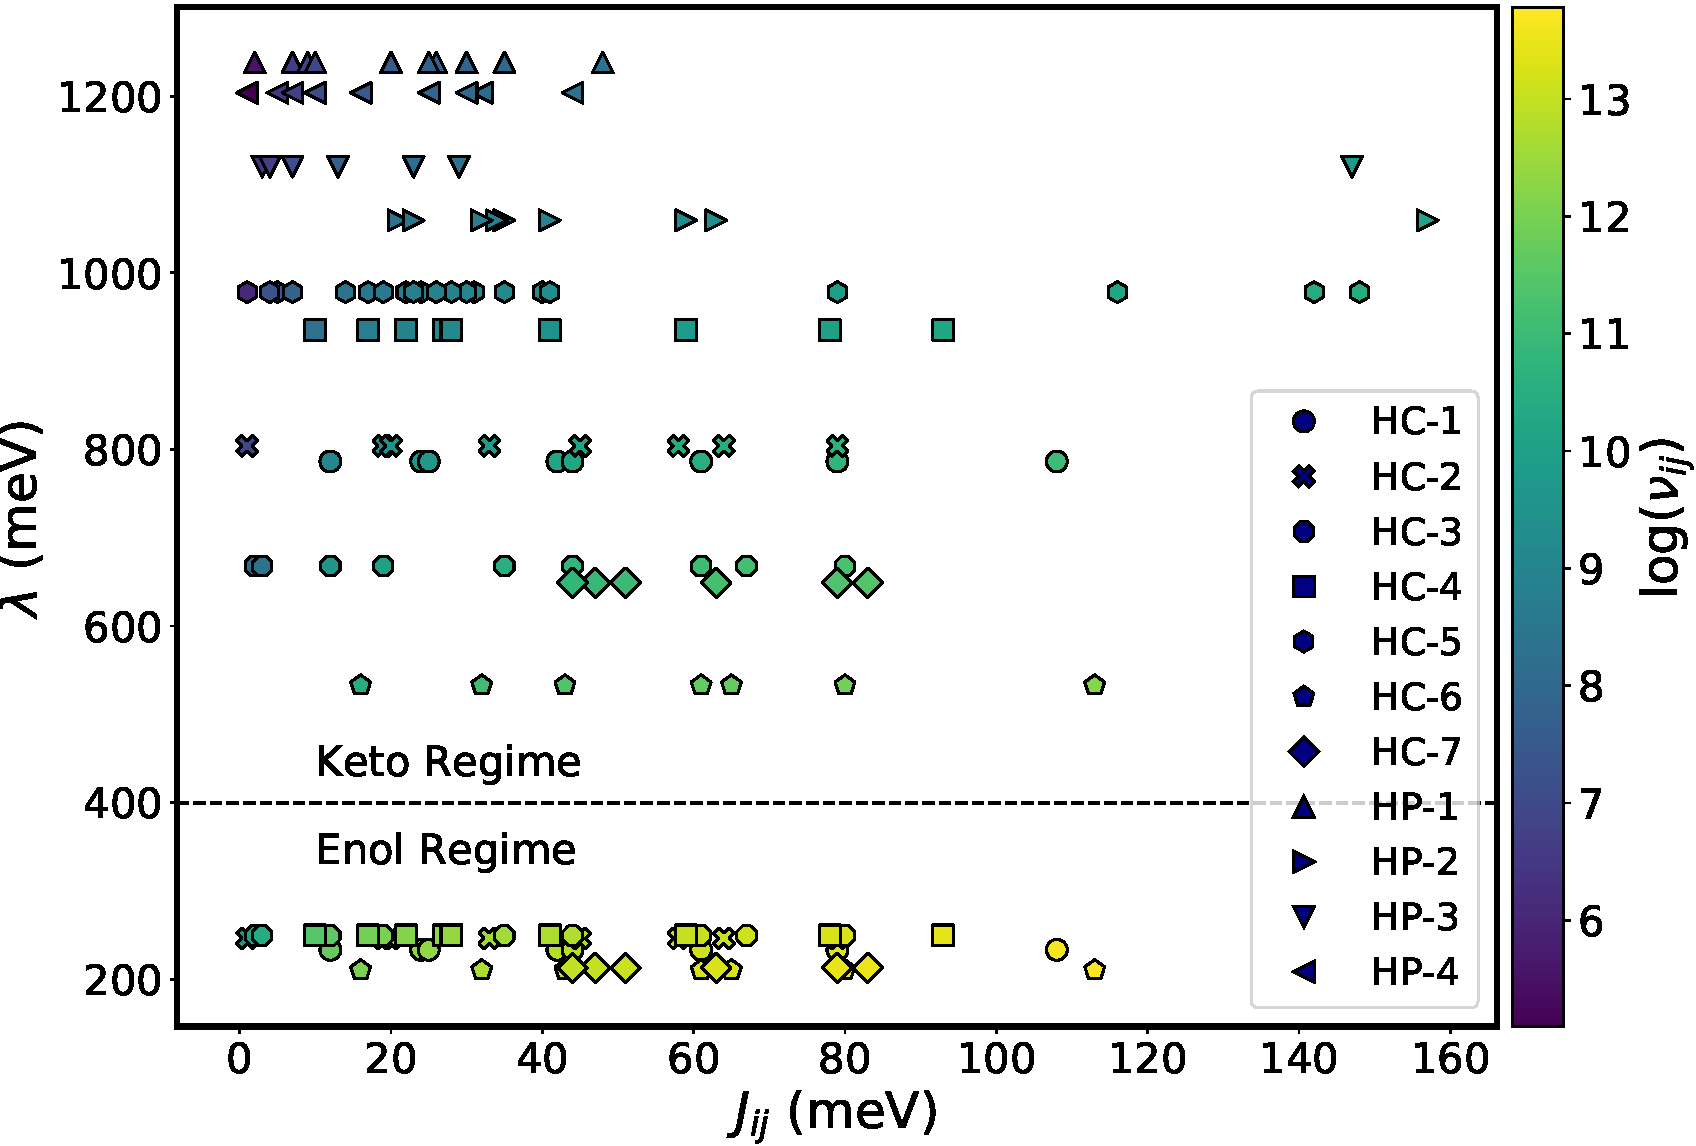
\includegraphics[width=0.8\linewidth]{5ConnectingCrystalStructure/marcus_3dscatter_vdw.pdf}
  \caption[Exciton hopping rates]{Colourmap of the exciton hopping rate $\nu_{ij}$ on a log\textsubscript{10} scale, as a function of the exciton coupling $J_{ij}$ and the reorganisation energy $\lambda$, calculated \textit{via} Equation \ref{equation: marcus}.}
  \label{figure: marcus_scatter_vdw}
\end{figure}

\begin{table}[t]
    \centering
    \begin{tabular}{ccccc}
    \hline
     System & $\lambda_{A}$\Estar{} (meV) & $\lambda_{A}$\Kstar{} (meV) & $\nu_{max}$\Estar{} (s\textsuperscript{-1}) & $\nu_{max}$\Kstar{} (s\textsuperscript{-1})\\
    \hline
    \textbf{HC1} & 233 & 786 & \SI{4.19e13}{} &\SI{1.05e11}{} \\
    \textbf{HC2} & 246 & 804 & \SI{1.92e13}{} &\SI{4.66e10}{}  \\
    \textbf{HC3} & 249 & 668 & \SI{1.90e13}{} &\SI{1.98e11}{} \\
    \textbf{HC4} & 250 & 936 & \SI{2.56e13}{} &\SI{1.67e10}{} \\
    \textbf{HC5} & -   & 978 & - & \SI{2.73e10}{} \\
    \textbf{HC6} & 210 & 533 & \SI{6.03e13}{} &\SI{1.64e12}{} \\
    \textbf{HC7} & 213 & 649 & \SI{3.15e13}{} &\SI{2.59e11}{} \\
    \hline
    \textbf{HP1} & - & 1238 &- &\SI{2.03e8}{}  \\
    \textbf{HP2} & - & 1059 &- &\SI{1.34e10}{}  \\
    \textbf{HP3} & - & 1120 &- &\SI{6.30e9}{}  \\
    \textbf{HP4} & - & 1204 &- &\SI{2.41e8}{}  \\
    \hline
    
    \end{tabular}
    \caption[Reorganisation energies and larges exciton hopping rates]{Adiabatic reorganisation energies ($\lambda_{A}$) and largest hopping rates $\nu$ in the enol (where available) and keto channels for \textbf{HC} and \textbf{HP} systems.}
    \label{table: reorgs_rates}
\end{table}

To explore the hopping rate close to the Franck-Condon state for \textbf{HP} systems, we use the exemplar \textbf{HP1} and optimise the
face-face dimer chromophore in \szero{} and \sone{} states. In particular, we locate the cis-trans isomerised \Estar{} minimum which was located in vacuum in Section \ref{section: Connecting_Vacuum}. Geometric relaxation in \Estar{} in \textbf{HP1} affords a torsion in the bridging unsaturated C-C bond to a non-fluorescent state and a reorganisation energy of 2114 meV. As a direct consequence, the hopping rate for such a large $\lambda$ is \SI{3.24e4}{s^{-1}}. For comparison, the smallest hopping rate for \textbf{HC1} in \Estar{} is \SI{5.17e+11}{s^{-1}} and, using the same methodology as \textbf{HP1}, \SI{3.92e+11}{s^{-1}} in \textbf{HC5}. Exciton hopping is therefore reduced in \textbf{HP} due to the relatively small exciton coupling, helping to fulfil design rule two.


%%%%%%%%%%%%
%%%%%%%%%%%%
\section{Conclusions}\label{section: Connecting_Conclusions}
%%%%%%%%%%%%
%%%%%%%%%%%%
In this Chapter we have systematically evaluated the photo behaviour of a range of solid-state emitters based on the ESIPT mechanism. The design rules established in Chapters \ref{chapter:NRdecay} and \ref{chapter: Inter} have been scrutinised for an expanded range of compounds, increasing the scope of the study of ESIPT chromophores. In the \textbf{HC} family of compounds, AIE is witnessed for five of the seven compounds, with \ac{QE} ranging from 0.10 to 0.84. In the \textbf{HP} systems, which differ by containing only one aryl ring, all reported compounds are emissive in the solid state with \ac{QE} of 0.72-0.84. In each crystal structure, there exist a range of dimers each with their own excitonic profile. In the \textbf{HC} systems, the herringbone stacking is prominent, with exciton coupling enhanced by the two aryl rings promoting $\pi-\pi$ interactions which are mostly absent in their \textbf{HP} counterparts.  

In the \textbf{HC} compounds, after photoexcitation to the \sone{} state, exciton hopping in the enol tautomer will compete with ESIPT on account of minimal electron density loss on the phenol oxygen and the stability of the planar enol tautomer, which results in only a small reorganisation energy. Here the the hopping rate is several orders of magnitude larger than in the \Kstar{} state and will allow nonradiative dissipation of the excited state. Conversely in the \textbf{HP} compounds, and \textbf{HC5}, the electron density loss is increased on the oxygen and ESIPT is more favourable, coupled with the planar \Estar{} tautomer being unstable. The stability of the \Kstar{} state increases the reorganisation energy $\lambda$ of the chromophore and subsequently will increase the population of the ESIPT channel in these systems. The \Kstar{} state will be highly localised with minimal hopping. In \textbf{HC1}, emission from \Estar{} will increase unfavourable self-absorption and contribute to the lower quantum yield compared to \textbf{HP1}.

The \Kstar{} minimum takes a planer conformation in the solid state, which considerable oscillator strength for emission back to \szero{}. \textbf{HP1} has an energetically inaccessible MECI, as for \textbf{HC1}, whereas in \textbf{HC5} the MECI is energetically accessible. As for \textbf{HC1}, the MECI for \textbf{HP1} in the crystal takes a distorted, pyramidalised geometry and is energetically inaccessible in the decay path. As such, emission will occur from the planar \Kstar{} minimum for the \textbf{HP} compounds and with larger \ac{QE}, due to the increase in the population of the \Kstar{} channel. Such is the similarity in absorption and emission spectra in the \textbf{HP} family, this mechanism is expected to be independent of the substituents present in this study. 

These findings help to connect the electronic, molecular picture with the crystalline regime for organic light-emitting materials. In these ESIPT emitters, the intermolecular interactions dominate in the Franck-Condon regime at photoabsorption. From here, the electronic structure and the character of the excited state, inherently molecular properties, become dominant. The deconstruction of intra- and intermolecular factors here, connecting the chromophore with its crystal structure, offers a step forward in first principles design of solid state luminescent materials exploiting ESIPT.
